% ===========================================================================
% Statistical Shape Reconstruction of Worn Enamel Dentine Junction Surfaces
% in Primate Molars   --   two-column manuscript
%
% Compile:  latexmk -pdf main.tex
%   or:     pdflatex main && bibtex main && pdflatex main && pdflatex main
%
% LAYOUT NOTES
%   * Narrow tables use `table` with [H] and sit inside one column.
%   * Wide tables use `table*`, which spans both columns. Starred floats in
%     two-column mode can only be placed at the top of a page -- a LaTeX
%     restriction -- so [H] is deliberately NOT used on them.
% ===========================================================================

\documentclass[10pt,a4paper,twocolumn]{article}

% --- encoding & fonts ---
\usepackage[utf8]{inputenc}
\usepackage[T1]{fontenc}
\usepackage{lmodern}
\usepackage[english]{babel}

% --- maths ---
\usepackage{amsmath}
\usepackage{amssymb}
\usepackage{bm}

% --- tables ---
\usepackage{booktabs}
\usepackage{array}
\usepackage{tabularx}
\usepackage{multirow}
\usepackage{float}

% --- layout ---
\usepackage[margin=1.9cm,columnsep=0.68cm]{geometry}
\usepackage{microtype}
\usepackage{titlesec}
\usepackage{enumitem}
\usepackage[font=small,labelfont=bf,skip=4pt]{caption}
\usepackage{graphicx}
\graphicspath{{figures/}}

% Dense setting: indent paragraphs rather than separating them with space.
\setlength{\parskip}{0pt}
\setlength{\parindent}{1em}

\titleformat{\section}{\normalfont\large\bfseries\raggedright}{\thesection}{0.6em}{}
\titleformat{\subsection}{\normalfont\normalsize\bfseries\raggedright}{\thesubsection}{0.6em}{}
\titlespacing*{\section}{0pt}{1.5ex plus .2ex minus .2ex}{0.7ex}
\titlespacing*{\subsection}{0pt}{1.2ex plus .2ex minus .2ex}{0.45ex}
\setlist{nosep,leftmargin=1.3em,topsep=2pt,itemsep=2pt}

% --- colour & links ---
\usepackage{xcolor}
\definecolor{linkblue}{RGB}{0,74,124}
\usepackage[colorlinks=true,linkcolor=linkblue,citecolor=linkblue,
            urlcolor=linkblue]{hyperref}

% --- bibliography ---
\usepackage{natbib}
\bibliographystyle{plainnat}
\setlength{\bibsep}{1.5pt plus 0.2ex}

% ---------------------------------------------------------------------------
% TYPOGRAPHY IN A NARROW MEASURE
% Two columns are only ~8cm wide, so LaTeX's defaults produce widows, orphans
% and one-word last lines. These settings suppress them.
% ---------------------------------------------------------------------------
\widowpenalty=10000        % never leave the first line of a para at column foot
\clubpenalty=10000         % never leave the last line of a para at column head
\displaywidowpenalty=10000
\brokenpenalty=10000       % never break a hyphenated word across a column
\interlinepenalty=150      % discourage splitting a paragraph at all

% Line breaking: a narrow measure needs more slack, or TeX resorts to ugly
% spacing and overfull boxes.
\tolerance=1200
\emergencystretch=2em
\hyphenpenalty=150
\hbadness=2000             % quieten warnings for boxes we accept

% Stop paragraphs ending in a single short word on its own line: the last line
% must now fill at least a third of the column.
\setlength{\parfillskip}{0pt plus 0.67\columnwidth}

% Let columns end short rather than stretching inter-paragraph space to fill.
\raggedbottom

% Float placement. Defaults allow so few floats per page that a deferred one
% queues all the later ones behind it -- which is why the parameter table
% landed alone after the references. The dbl* counters govern the two-column
% (starred) floats specifically.
\setcounter{topnumber}{3}
\setcounter{totalnumber}{5}
\setcounter{dbltopnumber}{3}
\renewcommand{\topfraction}{0.9}
\renewcommand{\dbltopfraction}{0.9}
\renewcommand{\textfraction}{0.07}
\renewcommand{\floatpagefraction}{0.7}
\renewcommand{\dblfloatpagefraction}{0.7}

% --- convenience ---
\newcommand{\mm}{\,\mathrm{mm}}
\newcommand{\code}[1]{\texttt{#1}}
\newcolumntype{L}{>{\raggedright\arraybackslash}X}

\title{\vspace{-1.2em}\bfseries\large
       Statistical Shape Reconstruction of Worn Enamel Dentine\\
       Junction Surfaces in Primate Molars\vspace{-0.2em}}

% ---------------------------------------------------------------------------
% AUTHORS -- fill in. Superscripts index the affiliation list; add or remove
% entries as needed.
% ---------------------------------------------------------------------------
\author{\normalsize
  Jeethu Srinivas Amuthan\,$^{1}$ \quad
  [Author Two]\,$^{1}$ \quad
  [Author Three]\,$^{2}$ \quad
  [Author Four]\,$^{2}$\\[0.35em]
  \footnotesize $^{1}$[Department, Institution, City, Country] \quad
  $^{2}$[Department, Institution, City, Country]\\[0.15em]
  \footnotesize Corresponding author: \texttt{jeethusrini2604@gmail.com}
  \vspace{-0.4em}}

\date{}

% ===========================================================================
\begin{document}
% ===========================================================================

\twocolumn[
  \begin{@twocolumnfalse}
    \maketitle
    \begin{center}
    \begin{minipage}{0.93\textwidth}
      \small
      \noindent\textbf{Abstract.}
      Tooth wear erases the crown shape that dental anthropologists rely on to
      identify species and study diet. The enamel dentine junction (EDJ), the
      surface beneath the enamel on which the crown forms, lasts longer than the
      outer surface, but heavy wear eventually removes it as well, and current
      reconstruction methods recover only a few measurements and work well only
      on lightly worn teeth. We present an automated pipeline that rebuilds the
      complete original EDJ surface of upper left third molars from 3D scans of
      worn teeth, without placing landmarks by hand. It matches points across
      specimens, learns the normal range of tooth shape from unworn teeth, and
      fills in the anatomy that wear removed. We compare three approaches: a
      global shape model, a model built from the most similar unworn teeth, and a
      nonrigid fit that bends the model output onto the real scan. A worn tooth is
      mostly intact, so scoring the whole surface would reward a method that
      changes nothing. We therefore measure accuracy only on the region that wear
      removed, which is between 1 and 25\% of the crown. We tested the pipeline on
      80 artificially worn cases with known originals, covering Molnar wear stages
      3 to 6. On 64 cases from eight specimens the model had never seen, sampled at
      10,000 points per tooth, the global shape model restored worn anatomy with a
      root mean square error of $0.27\mm$. The nonrigid fit matched the intact
      surface most closely but was 35\% worse on the worn region, because its warp
      pulled the rebuilt cusps back toward the worn surface. On a smaller series
      sampled ten times more densely, the nonrigid fit was the most accurate
      method, at $0.10\mm$. Error grows with wear and rises sharply at Molnar stage
      6, which marks the practical limit of the method. Checking every
      registration showed that a tooth turned half a turn during alignment can
      silently corrupt a shape model, and we describe the check that caught it. We
      also describe how the pipeline is being packaged as a library that documents
      the settings available at each step.

      \medskip
      \noindent\textbf{Keywords:} enamel dentine junction; statistical shape
      model; tooth wear; dental anthropology; surface reconstruction; coherent
      point drift; Molnar wear stages.
    \end{minipage}
    \end{center}
    \vspace{1.4em}
  \end{@twocolumnfalse}
]

% ===========================================================================
\section{Introduction}
\label{sec:intro}
% ===========================================================================

Teeth are the most frequently recovered and best preserved elements of the
vertebrate skeleton. Enamel is the hardest tissue the body produces, so teeth
survive burial, fossilisation and taphonomic processes that destroy bone, and in
many assemblages they are the only elements available in usable numbers. Molar
crown morphology carries much of the taxonomic, phylogenetic and dietary signal
that dental anthropology relies on: cusp number, position and relative height,
the configuration of ridges and fissures between them, and the shape of the
occlusal basin are all used to distinguish taxa and to reconstruct diet.

Wear progressively erases that signal. Mastication, abrasive diet and bruxism
strip enamel from the occlusal surface throughout life, and the process is
cumulative and irreversible. In the early stages wear planes off the enamel
crests while leaving the underlying architecture intact; later it perforates the
enamel cap and exposes dentine; eventually it truncates the cusps themselves. An
individual old enough to be interesting for life-history questions is often worn
past the point where the traits of interest can be scored.

\subsection{Why the enamel dentine junction}

The enamel dentine junction (EDJ) is the interface between the enamel cap and
the dentine core beneath it. It is not an incidental boundary: it is the
developmental template on which enamel is deposited. During odontogenesis the
inner enamel epithelium folds into the shape the future crown will take,
ameloblasts differentiate along it, and enamel is laid down outward from that
surface. The EDJ therefore records crown form at the moment of its formation,
and because it is sealed beneath the enamel and never remodelled during life, it
retains that record while the outer surface is worn away. This is why EDJ
morphology has become a standard target for taxonomic and phylogenetic work on
worn and fossil material \citep{skinner2008traits,skinner2008edj}: dentine horn
position and relative height survive attrition that has erased the corresponding
features from the outer enamel surface.

But the EDJ is only \emph{relatively} robust. Once wear breaches the enamel cap
it begins to remove dentine, and the dentine horns, precisely the features
that carry the signal, are truncated. The specimens most in need of
morphological analysis, the old individuals and the heavily worn fossils, are
exactly those whose EDJ can no longer be measured directly. Recovering the
pre-wear EDJ surface from a worn one is therefore a problem worth solving, and
it is the problem this paper addresses.

\subsection{Existing approaches and their limits}

Anthropology has addressed crown reconstruction with methods that are largely
manual and largely two-dimensional. The Profile, Polynomial and Pen Tool methods
each reconstruct a missing crown portion by extending the surviving outline:
Profile by mirroring an unworn homologue, Polynomial by fitting a curve to the
surviving enamel and extrapolating it, Pen Tool by manual tracing. A systematic
comparison \citep{ohara2022reconstructing} found all three reliable only for
relatively unworn crowns, with Profile and Polynomial preferred as wear
increases, and recommended different methods depending on whether crown height
or enamel thickness is the quantity of interest. More recent work predicts EDJ
cusp height in worn lower molars from morphometric variables using Random Forest
and regression ensembles \citep{cuspml2026}.

These approaches share two limitations. First, they recover a small number of
scalar measurements (crown height, cuspal enamel thickness, horn-tip height)
rather than a surface. A scalar is enough to test a specific hypothesis about
crown height, but not to compare occlusal topography, run a geometric
morphometric analysis, or render the reconstructed tooth. Second, they require
operator decisions, such as where to place a profile plane or which points to
include in a polynomial fit, that are difficult to standardise across laboratories and
that make inter-operator agreement a live concern.

\subsection{The statistical shape model alternative}

A statistical shape model (SSM) offers a different route \citep{cootes1995asm}.
The idea is to learn, from a sample of complete specimens, what shapes that
anatomy actually takes, and then to use that learned distribution to fill in
whatever is missing from an incomplete specimen. Because the model knows the
range of plausible crown forms, it can propose a completion that is consistent
with real anatomy rather than with an arbitrary mathematical extrapolation.

Three properties make this attractive here. The output is a complete surface, not
a set of measurements, so any downstream analysis that could have been run on the
original tooth can be run on the reconstruction. The procedure is deterministic
given its parameters, so two laboratories running the same configuration on the
same input obtain the same result. And the reconstruction is constrained by the
training sample, so it cannot invent a crown form that no real tooth exhibits.

\subsection{This paper}

We report such a pipeline for primate upper left third molar (ULM3) EDJ surfaces.
Three reconstruction strategies are implemented against a shared correspondence
stage so that they can be compared directly: a \emph{global} shape model built
from all unworn specimens, a per-specimen \emph{neighborhood} model built from
the anatomically nearest unworn teeth, and a \emph{non-rigid fit} that warps the
model output back onto the observed scan under a confidence gate.

As much as the reconstruction itself, this paper is about a validation protocol
that does not flatter the method. Reconstruction quality in this domain is easy
to overstate, for a structural reason: a worn tooth is mostly intact. Even at
severe wear the damaged region is a minority of the crown surface, so any error
metric averaged over the whole tooth is dominated by surface that was never
damaged in the first place. A method that returns its input completely unchanged
will score well on such a metric while restoring nothing at all. We therefore
score restoration on a shared, method-agnostic mask of the anatomy wear actually
removed, and report whole-surface and fidelity-to-scan figures only as supporting
evidence, explicitly excluded from the ranking.

\paragraph{Contributions.}
\begin{enumerate}
  \item An end-to-end, parameterised pipeline from raw worn mesh to reconstructed
        EDJ surface, requiring no manual landmarking at any stage.
  \item Three reconstruction strategies sharing one correspondence stage, so
        differences between them are attributable to the reconstruction step
        rather than to preprocessing.
  \item A three-layer validation protocol with an explicit worn-region mask,
        applied to two independent artificially worn series (16 and 64 cases)
        with known ground truth, across Molnar wear stages 3 to 6.
  \item A characterisation of where these methods fail: at severe wear, where
        we identify the practical limit of the approach, and at low point
        density, where the non-rigid fit distorts the anatomy it rebuilds.
  \item Two checks that other shape-model studies can reuse: a registration
        check that catches teeth registered in the wrong orientation, and a wear
        mask that does not mistake sparse sampling for missing anatomy.
\end{enumerate}

% ===========================================================================
\section{Background: shape models in one page}
\label{sec:background}
% ===========================================================================

This section sets out the machinery in accessible terms; readers familiar with
statistical shape modelling can skip to \S\ref{sec:related}.

\paragraph{Correspondence.}
Shape statistics require \emph{homology}: point $i$ must denote the same
anatomical location on every specimen. Two meshes of the same tooth type are not
automatically comparable, because a mesh is just a list of vertices in whatever
order the scanner produced, and two scans of the same tooth will have different
vertex counts and orderings. Establishing correspondence means producing, for
every specimen, a point cloud of identical size in which the $i$th point sits on
the same anatomical feature. Traditionally this was done by placing landmarks by
hand. We do it automatically (\S\ref{sec:corr}).

\paragraph{Shape space.}
Once every specimen is represented by $N$ corresponded points in three
dimensions, it can be flattened into a single vector of length $3N$. A specimen
is then one \emph{point} in a $3N$-dimensional space, and a collection of
specimens is a cloud of points in that space. Anatomy is highly constrained
(teeth do not vary arbitrarily), so that cloud occupies only a thin subregion of
the full space.

\paragraph{Principal component analysis.}
PCA finds the directions along which the cloud actually varies. The mean shape
$\bm{\mu}$ is the average of the training specimens; the principal modes
$\mathbf{V}$ are the directions of greatest variance, ordered by how much
variance each explains. A shape is then approximated as
$\mathbf{x}(\mathbf{b}) = \bm{\mu} + \mathbf{V}\mathbf{b}$, where the
coefficients $\mathbf{b}$ say how far along each mode to travel. Because anatomy
is constrained, a handful of modes typically suffices: in our EDJ model the first
mode alone accounts for $45.5\%$ of total variance and the first two for
$60.0\%$.

\paragraph{Fitting a partial shape.}
The reconstruction step exploits an asymmetry. The coefficients $\mathbf{b}$ are
shared across the whole shape, so they can be estimated from \emph{any} subset of
the points, in particular from the part of the worn tooth that survives. Once
$\mathbf{b}$ is known, evaluating $\bm{\mu} + \mathbf{V}\mathbf{b}$ gives
coordinates for \emph{every} point, including those in the worn region that were
never observed. That is how the model supplies the missing anatomy: not by
extrapolating the surviving surface, but by asking which plausible complete tooth
best explains what survives.
% ===========================================================================
\section{Related work}
\label{sec:related}
% ===========================================================================

\paragraph{Worn teeth in anthropology.}
\citet{ohara2022reconstructing} compared the Profile, Polynomial and Pen Tool
methods for crown height and enamel thickness, concluding that accurate
reconstruction is limited to relatively unworn crowns, with method choice
depending on the measurement of interest. Micro-computed tomography has been used
to reconstruct worn or broken cusps non-destructively and to check for internal
cracks before physical casting. A recent machine-learning pipeline predicts EDJ
horn-tip height in worn lower molars from height, area and volume variables
using Random Forest and regression ensembles \citep{cuspml2026}. All of these
target scalar measurements; none returns a reconstructed surface, which is the
gap this work addresses.

\paragraph{Statistical shape models of teeth.}
\citet{buchaillard2007tooth} built 3D statistical models for tooth surface
reconstruction, reporting mean surface error below $0.2\mm$ with five principal
components and below $0.1\mm$ with thirteen, which established that a
modest number of modes suffices for dental crown geometry.
\citet{woods2017ssm} applied SSM to 27 mandibular canines spanning modern,
Anglo-Saxon and Roman samples, reporting reconstruction error below $0.2\mm$
after five components, roughly $0.7\%$ of mean canine length, with the first five
capturing about $75\%$ of variance. Their work is the closest methodological
precedent for ours: high-density correspondence, PCA, archaeological material.
Gaussian process morphable models \citep{luthi2018gpmm} generalise the PCA
formulation to continuous covariance functions, allowing deformation beyond the
linear span of the training set, and underpin much of the modern posterior
shape-completion literature.

\paragraph{Learning-based dental reconstruction.}
A separate line of work reconstructs teeth from 2D inputs. TeethDreamer
\citep{teethdreamer2024} generates 3D teeth from five intra-oral photographs
using a diffusion prior to hallucinate novel views, then neural surface
reconstruction. Occudent \citep{occudent2023} recovers 3D teeth from a single
panoramic radiograph with neural implicit functions. These solve a substantially
harder and more underdetermined problem, inferring 3D geometry, scale and
tooth identity from 2D projections, and their reported errors are
correspondingly larger. \S\ref{sec:imagebased} explains why we do not tabulate
them alongside our results.

\paragraph{Positioning.}
Our work sits between these strands: the anthropological target (EDJ morphology
of worn molars, staged on a standard wear scale) combined with the methodological
apparatus of dental SSM (dense automatic correspondence, PCA priors, posterior
fitting), evaluated on artificially worn series where the true pre-wear surface
is known. To our knowledge this combination has not previously been reported:
surface-level EDJ reconstruction, with no manual landmarks, validated against
ground truth across a graded wear series.

% ===========================================================================
\section{Materials}
\label{sec:materials}
% ===========================================================================

All specimens are upper left third molars (ULM3). EDJ surfaces were extracted
from micro-CT and exported as triangle meshes in millimetres. Two independent
datasets are used (Table~\ref{tab:specimens}), referred to throughout as the
\textbf{EDJ series} and the \textbf{ULM series} after their respective naming
conventions.

\begin{table}[H]
\centering
\caption{Specimen inventory. For the ULM series the eight test specimens are
  excluded from the 90-tooth training pool, so every ULM reconstruction is of a
  specimen the model has never seen. One of the 18 scanned EDJ training teeth
  (\code{n0307}) failed the registration check and is excluded
  (\S\ref{sec:regcheck}).}
\label{tab:specimens}
\footnotesize
\begin{tabularx}{\columnwidth}{@{}>{\raggedright\arraybackslash}p{1.45cm}Lr@{}}
\toprule
\textbf{Set} & \textbf{Role} & \textbf{$n$} \\
\midrule
EDJ train & unworn, SSM training & 17 \\
EDJ test  & artificially worn (TEST1, TEST2) & 2$\times$8 \\
EDJ natural & naturally worn, no original & 9 (5 used) \\
ULM train & unworn, SSM training & 90 \\
ULM test  & artificially worn, held out & 8$\times$8 \\
\midrule
\multicolumn{3}{@{}l}{\itshape Wear level $\rightarrow$ Molnar stage} \\
\multicolumn{3}{@{}l}{L0--L1 $\rightarrow$ 3\quad L2--L3 $\rightarrow$ 4\quad
                      L4--L5 $\rightarrow$ 5\quad L6--L7 $\rightarrow$ 6} \\
\bottomrule
\end{tabularx}
\end{table}

\subsection{Why artificial wear}

Ground truth for a \emph{naturally} worn tooth does not exist. The pre-wear
surface is precisely what attrition destroyed, so for a real worn specimen there
is nothing to compare a reconstruction against, and any evaluation reduces to
expert judgement of plausibility. This is the central methodological obstacle in
the field, and it is why published reconstruction methods are often validated
only on lightly worn teeth where the missing portion can be inferred by other
means.

We sidestep it with artificially worn series. Each source specimen, a complete
unworn tooth, was progressively worn in eight digital steps, producing eight
worn variants whose true pre-wear surface is known exactly, because it is the
original mesh the series was generated from. This gives matched (worn, original)
pairs at graded severity, and makes quantitative validation possible. The
trade-off is that digital wear is not identical to natural attrition, a
limitation we return to in \S\ref{sec:limitations}.

\subsection{Wear staging}

The eight steps map onto \textbf{Molnar wear stages 3 to 6}
\citep{molnar1971wear}, two steps per stage, so results can be read against a
standard anthropological wear scale rather than an arbitrary index. Molnar's
scale runs from 1 to 8 and describes progressive dentine exposure: stage 3 marks the
first substantial dentine patches, stage 4 their coalescence, stage 5 extensive
dentine exposure with enamel confined to the rim, and stage 6 near-complete loss
of the occlusal enamel. Our series therefore spans the range over which EDJ-based
analysis normally becomes difficult, which is exactly where a reconstruction
method needs to be tested.

EDJ ground-truth meshes are \code{n0245} (TEST1) and \code{n0257} (TEST2). ULM
test specimens are N1063, N332, N4, N459, N705, N726, N728 and N891.

The EDJ series also includes nine naturally worn teeth. They have no unworn
original, so they cannot be scored; we use them only to show how the pipeline
behaves on natural wear (\S\ref{sec:natural}).

% ===========================================================================
\section{Methods}
\label{sec:methods}
% ===========================================================================

The pipeline runs in three stages: establish correspondence across all specimens
(\S\ref{sec:corr}), reconstruct each worn tooth (\S\ref{sec:global} to
\S\ref{sec:nonrigid}), then evaluate (\S\ref{sec:protocol}). The three
reconstruction strategies are independent alternatives consuming the same
Stage~1 output, so any subset can be run alone and differences between them are
attributable to the reconstruction step alone. Figure~\ref{fig:pipeline} follows
one worn EDJ specimen, not part of the training set, through every step.

\begin{figure*}[!t]
\centering
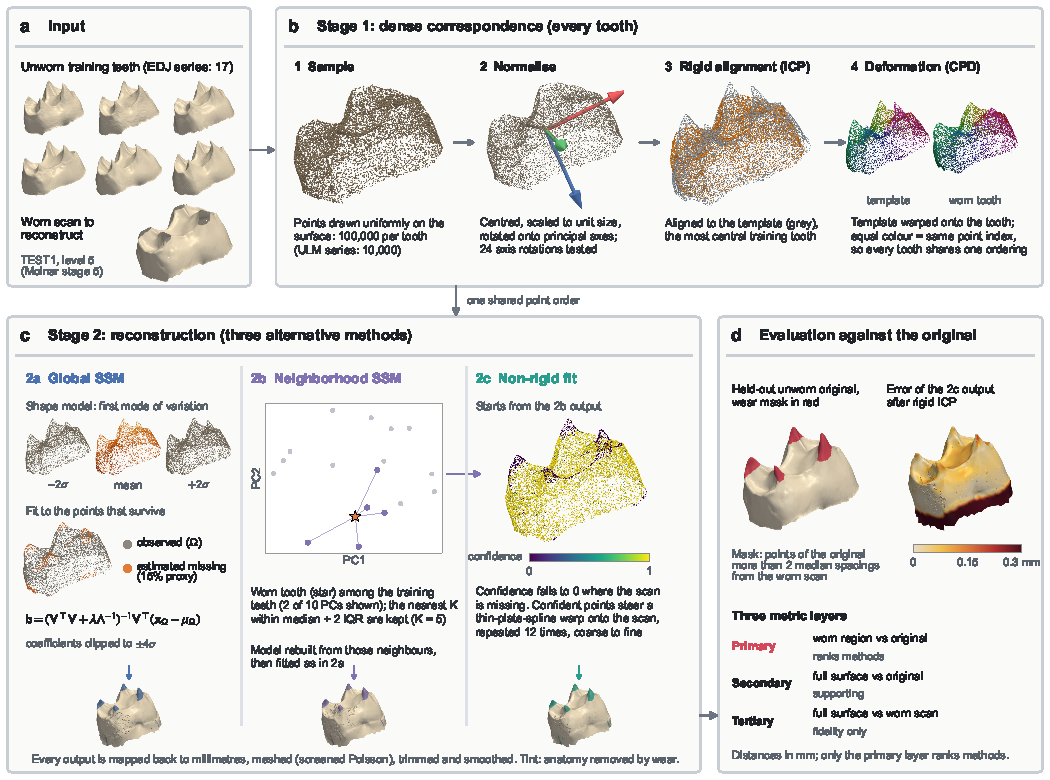
\includegraphics[width=\textwidth]{fig_pipeline_edj.pdf}
\caption{The reconstruction pipeline, shown on one EDJ specimen that is not in the
  training set (TEST1, wear level 5, Molnar stage 5); every image is rendered from
  the pipeline's own intermediate files for this case. \textbf{(a)} Inputs: six of
  the 17 unworn training teeth and the worn scan to be reconstructed. Artificial
  wear only deletes surface, so the worn scan is drawn as the original surface
  with the worn region removed. \textbf{(b)} Stage~1 gives every tooth the same
  ordered set of points. Surface points are sampled, normalised for position, size
  and orientation, and rigidly aligned to an automatically chosen template, which
  coherent point drift then deforms onto the tooth; equal colours mark the same
  point on the template and on the worn tooth. \textbf{(c)} Stage~2 offers three
  alternative reconstructions. The global shape model (2a) is fitted to the points
  treated as observed and supplies the rest. The neighborhood model (2b) rebuilds
  the shape model from the five training teeth nearest the worn tooth, shown here on
  two of the ten principal components used for the selection. The non-rigid fit (2c)
  starts from the 2b output and warps it onto the scan wherever confidence is high.
  Each output is meshed in millimetres, and the tint marks the anatomy that wear
  removed. \textbf{(d)} Outputs are scored against the held-out original. The wear
  mask (red) defines the primary metric layer, and the error map shows the distance
  from the non-rigid output to the original after rigid alignment.}
\label{fig:pipeline}
\end{figure*}

\subsection{Stage 1: dense correspondence}
\label{sec:corr}

We obtain homologous points without manual landmarking, following the logic of
automated point-cloud landmarking approaches such as ALPACA
\citep{porto2021alpaca}. The stage has four steps.

\begin{enumerate}
  \item \textbf{Sample.} Points are drawn uniformly from each mesh surface:
        $100{,}000$ for the EDJ set, $10{,}000$ for the ULM set, reflecting the
        different mesh resolutions of the two datasets. Sampling from the
        \emph{surface} rather than taking mesh vertices removes any dependence on
        how the scanner happened to tessellate the tooth.
  \item \textbf{Normalise.} Each cloud is centred on its centroid, divided by its
        bounding-box diagonal to remove size, and rotated onto its principal
        axes. Removing size is deliberate: we model \emph{shape}, and absolute
        tooth size varies with sex, population and individual without carrying
        the morphological signal of interest. The rotation step needs care.
        The sign of a PCA axis is mathematically arbitrary (an axis and its
        negation are equally valid), and a crown is nearly as long as it is
        wide, so PCA can also order the two horizontal axes either way. Two teeth
        can therefore be normalised into orientations that differ by a half or a
        quarter turn. We try all 24 rotations that map the principal axes onto
        themselves, align each to the template by iterative closest point run
        to convergence, and keep the rotation with the smallest two-way surface
        distance to the template. The template-to-tooth direction is trimmed to
        its closest 85\% of points, so that anatomy missing from a worn scan does
        not count against the correct orientation. Mirror images are never
        considered, because reflecting a tooth changes its anatomy. Without this
        step registration can begin half a turn out and never recover, producing
        a corresponded cloud that is anatomically scrambled
        (\S\ref{sec:regcheck}).
  \item \textbf{Rigid align.} Iterative closest point \citep{besl1992icp} aligns
        each normalised cloud to a template, chosen automatically as the most
        central specimen in the sample so that no tooth is privileged by an
        arbitrary choice of reference.
  \item \textbf{Deform.} Coherent point drift \citep{myronenko2010cpd} warps the
        \emph{template} onto each target. The direction matters: because the
        template's own point ordering travels with it, the deformed template
        \emph{is} the correspondence: its $i$th point now sits at the
        anatomically corresponding location on the target. CPD treats the
        registration as fitting a Gaussian mixture with a motion-coherence
        constraint, which keeps neighbouring points moving together and prevents
        the deformation from tearing. For high point counts CPD is run on a
        subset and the resulting displacement field interpolated back to the full
        cloud, since CPD cost grows with the square of the point count.
\end{enumerate}

The output is one cloud per specimen, all of identical size and shared ordering.

\paragraph{Registration check.}
\label{sec:regcheck}
Every registration was checked in two ways. First, each tooth's final
orientation was compared with all 24 axis rotations after converged alignment to
the template; a correct registration is the best of them. Second, for the
artificially worn series, the corresponded points of every worn scan were
compared with those of its own unworn original in millimetres: if both are
registered consistently, point $i$ sits on the same anatomy in both, apart from
the cusps that wear removed. On the ULM series the median offset grows smoothly
with wear, from $0.09\mm$ at level~0 to $0.48\mm$ at level~7, and never
exceeds $0.66\mm$; a tooth registered half a turn out shows offsets of 4 to
$8\mm$.

The check changed this study. An earlier version of the orientation step chose
among candidates by the fraction of points within a fixed distance of the
template, a score that reaches 1.0 for several orientations at once and so
cannot separate a correct orientation from one turned half a turn; it also
allowed mirror images. That version had left 51 of the 90 ULM training teeth and
five of the eight held-out specimens half a turn out relative to the template,
and had mirrored three teeth. The half-turn teeth formed a separate group in
shape space, so the first mode of the ULM shape model described registration
orientation rather than anatomy. All ULM teeth were re-registered with the
orientation step described above. For three training teeth the full alignment
that follows the orientation search settled in a clearly worse position than the
search itself had found (fit score about four times the typical value), so the
alignment is now restarted from the search result whenever that happens. Every
result in this paper uses the re-registered data. On the EDJ series 17 of the 18 training teeth passed; the
remaining tooth, \code{n0307}, was turned half a turn and could not be
re-registered at the original settings on the hardware available, so it is
excluded from the EDJ models, which are therefore built from 17 teeth.

The check also covered the mapping back to millimetres. For the EDJ series, the
normalisation parameters stored by the original Stage~1 run did not reproduce the
aligned clouds exactly; mapping outputs back with them rotated each reconstruction
by 1 to 17 degrees. The rigid alignment before scoring (\S\ref{sec:protocol})
undid this at most wear levels but not at level~7, where it had inflated the error.
All outputs are now mapped with the exact transform described under Surface output.
Of the nine naturally worn teeth (\S\ref{sec:materials}), five passed the
registration check; three were registered half a turn out and one fits the
template poorly in every orientation, so these four are not reconstructed here.

\subsection{Stage 2a: global shape model}
\label{sec:global}

Stacking the corresponded unworn teeth gives a mean shape $\bm{\mu}$ and, by PCA,
modes $\mathbf{V}$ with variances $\bm{\Lambda}$. Fitting a worn tooth means
finding the coefficients $\mathbf{b}$ that best explain the points that
\emph{survive}, and letting the model supply the rest. With $\Omega$ the observed
subset, $\mathbf{b}$ follows from Tikhonov-regularised least squares:
\begin{equation}
  \mathbf{b} =
  \bigl(\mathbf{V}^{\!\top}\mathbf{V} + \lambda\bm{\Lambda}^{-1}\bigr)^{-1}
  \mathbf{V}^{\!\top}\bigl(\mathbf{x}_\Omega - \bm{\mu}_\Omega\bigr).
  \label{eq:fit}
\end{equation}

The regularisation term is what stops a partial observation producing a wild
model. Fitting from incomplete data is under-determined: many coefficient vectors
explain the surviving surface about equally well, and an unregularised solution
will happily pick one that behaves absurdly in the unobserved region.
$\lambda\bm{\Lambda}^{-1}$ penalises each mode in inverse proportion to its
variance in the training sample, so rare deformations must earn their place
against strong evidence while common ones are cheap. Coefficients are
additionally clipped to $\pm4\sigma$, a hard bound preventing the fit from
straying outside the range of real anatomy.

On the EDJ set, 17 training teeth yield 14 modes at $99.3\%$ of total variance
(PC1 alone $45.5\%$; PC1 and PC2 together $60.0\%$; $95\%$ reached at mode~10).
On the ULM set, 90 teeth yield 30 modes at $99.0\%$ (PC1 $27.2\%$; $95\%$ at
mode~18).

\paragraph{Identifying the missing region.}
Equation~\eqref{eq:fit} requires knowing which points are observed. For a real
worn tooth that is unknown, so it is estimated, in the same way for every
reconstruction reported here; the evaluation never gives a method the true worn
region. The estimate asks where the model predicts anatomy that the scan does not
have. Starting from the mean shape, the fixed fraction of model points lying
farthest from the worn scan (\code{proxy\_missing\_fraction}, 15\%) is treated
as missing. The model is then fitted to the remaining points, distances are
recomputed from the fitted shape, and the two steps repeat until the selection
stops changing. Where the tooth is intact the fitted shape lies on the scan;
where wear removed material it predicts cusps with no scan surface nearby.

We checked this estimate against the region that wear actually removed on the
held-out ULM series. Of the points it treats as missing, 90\% are truly missing
at level~7 and 62\% at level~4 (averaged over all levels, precision 0.49 and
recall 0.67). At levels~0 and~1 precision is necessarily low, because wear has
removed only about 2\% of the crown while 15\% is always selected. An earlier
heuristic that ranked points by height below the \emph{mean} shape reached a
precision of only 0.11 and recall of 0.10, because it mostly picked places where
a specimen simply differs from the average tooth.

The fraction is the single most
consequential parameter in the pipeline and the one most deserving of attention
from anyone adopting it. Set too high, healthy anatomy is discarded and replaced
by model estimate; set too low, genuinely worn anatomy is treated as observed and
the fit is dragged down toward the worn surface.

\paragraph{Non-rigid refinement.}
The raw model output is only as detailed as the model allows, and will not match
the observed surface exactly even where that surface survives. A refinement step
therefore snaps observed points back to their measured positions and carries the
resulting correction into the reconstructed region by inverse-distance-weighted
interpolation, so that filled anatomy joins real anatomy without a visible seam.

\subsection{Stage 2b: neighborhood shape model}
\label{sec:nbr}

A model built from all unworn teeth describes the \emph{population}, and its mean
is the population mean. If a worn specimen belongs to a morphological subgroup,
such as a population with distinctive cusp proportions, then fitting it against
a population prior pulls its reconstruction toward a centroid it does not belong
to. The neighborhood variant addresses this by rebuilding the model per specimen:

\begin{enumerate}
  \item Project all unworn teeth into a low-dimensional PCA space.
  \item Set an adaptive threshold at $\mathrm{median} + 2\,\mathrm{IQR}$ of the
        pairwise distances among them. Deriving the threshold from the sample's
        own spread, rather than fixing it, is what makes the criterion portable
        across datasets of different morphological diversity.
  \item Project the worn tooth into the same space and select every unworn tooth
        within that threshold, capped at $K$ ($K=5$ for the EDJ series and
        $K=10$ for the ULM series).
  \item Build the SSM from those neighbours alone, falling back to the global
        model if none qualifies.
\end{enumerate}

Everything downstream is identical. The cost is fewer modes (a $K$-neighbour
model has at most $K-1$), so the local model trades expressive range for a
tighter, more relevant prior. Whether that trade pays off is an empirical
question; \S\ref{sec:tie} reports that on this material it pays off only
slightly.

\subsection{Stage 2c: non-rigid fit}
\label{sec:nonrigid}

Both SSM variants produce a surface that is anatomically complete but limited in
detail by the model's mode count. The non-rigid fit takes such a reconstruction (in this study, the Neighborhood
SSM output) and warps it back onto the real scan, keeping model anatomy only where the scan has
nothing to say. After rigid alignment, each reconstruction point's distance to
the nearest scan point is converted into a \emph{confidence}: high where the scan
is present and falling smoothly to zero where it is absent, as in the worn
region, where by definition no scan surface exists. Confident points then become
landmarks for a thin-plate-spline warp \citep{bookstein1989tps} of the whole
reconstruction, and the process repeats coarse-to-fine, with the distance band
tightening and the smoothness penalty relaxing each round so that early
iterations fix gross alignment and later ones recover detail.

Where the tooth is intact the output converges on the real measured surface;
where wear removed material there are no confident landmarks, and the model's
anatomy is meant to be retained. The warp is smooth, however, so some of the pull
from nearby confident points reaches that region, and how much depends on point
density (\S\ref{sec:density}). Crucially, no scan points enter the output. Only
the warped reconstruction is returned, so scanning noise, holes and lace
artefacts are not inherited.

\subsection{Surface output}

Reconstructed clouds are mapped back to the original millimetre coordinate frame
with the exact similarity transform between each tooth's Stage~1 sample and its
aligned cloud, which Stage~1 saves in the same point order. They are then meshed with screened Poisson
reconstruction \citep{kazhdan2013poisson}, trimmed at the $1\%$ density quantile
to remove the extrapolated fringe Poisson produces at surface boundaries, and
Taubin-smoothed \citep{taubin1995smoothing}, which attenuates high-frequency
noise without the shrinkage that naive Laplacian smoothing causes. Mesh handling
uses Open3D \citep{zhou2018open3d}.
% ===========================================================================
\section{Evaluation protocol}
\label{sec:protocol}
% ===========================================================================

Ground truth is the unworn original, never the worn scan. Each reconstruction is
taken in millimetre space and rigidly aligned to the original before any distance
is computed, so that residual pose differences are not counted as shape error.

\subsection{The shared wear mask}

Restoration must be scored on the anatomy that wear actually removed. We identify
it on the ground-truth surface, sampled at $120{,}000$ points: a point of the
original is worn if it lies farther from the worn surface than twice the
original's median point spacing plus one and a half times the spacing of the
sample that represents the worn surface ($100{,}000$ points for both series). The
second term matters. A finite sample of a surface leaves gaps, and without it the
gaps themselves read as wear: resampling an \emph{unworn} tooth flags about
10\% of its surface as worn at $100{,}000$ points and about 80\% at
$10{,}000$ points, whereas with it the figure is 0.01\%. Where exact worn meshes
are available, the mask agrees with an exact point-to-surface mask on 92 to 99\%
of points. The worn region defined this way covers 2.3\% of the crown at level~0
rising to 24.4\% at level~7 on the ULM series, and 0.6 to 12.3\% on the EDJ
series (Table~\ref{tab:levels}).

Two properties matter. The mask is computed from the ground truth and the worn
scan only, so it is \textbf{method-agnostic}: no method is scored on its own idea
of what it repaired, which would let a conservative method look good by
attempting little. And it is \textbf{shared}: every method is scored on exactly
the same point set, so the comparison between columns is like for like.

\subsection{Why one number is not enough}

\begin{table*}[!t]
\centering
\caption{The three metric layers, what each compares, and the question each
  answers. Only the primary layer is used for ranking.}
\label{tab:layers}
\small
\begin{tabularx}{\textwidth}{@{}>{\raggedright\arraybackslash}p{2.0cm}>{\raggedright\arraybackslash}p{4.6cm}L>{\raggedright\arraybackslash}p{2.8cm}@{}}
\toprule
\textbf{Layer} & \textbf{Compares} & \textbf{Question it answers} & \textbf{Used for ranking?} \\
\midrule
\textbf{Primary} & worn region $\to$ original &
  Did the missing anatomy actually come back? & \textbf{Yes} \\
\textbf{Secondary} & full surface $\leftrightarrow$ original &
  How close is the whole reconstruction to a healthy tooth? & Supporting only \\
\textbf{Tertiary} & full surface $\leftrightarrow$ worn scan &
  Was the intact enamel preserved rather than distorted? &
  \textbf{No}, fidelity only \\
\bottomrule
\end{tabularx}
\end{table*}

A worn crown is mostly undamaged, so a single aggregate number is dominated by
the easy part of the problem. Table~\ref{tab:layers} separates three questions
that a single metric would conflate.

The tertiary layer illustrates the danger most sharply. It compares the
reconstruction against the \emph{worn input}, and a method that returned its
input completely unchanged would score a perfect zero on it while restoring
nothing whatsoever. Any ranking built on that layer is therefore inverted with
respect to the question actually being asked. The secondary layer is less
extreme but suffers the same bias in milder form: because the intact region
dominates by area, a method that reproduces intact enamel well and fills the worn
region badly can still post an excellent full-surface score. Only the primary
layer isolates the part of the problem that is genuinely hard.

This concern is not specific to dentistry. \citet{tatarchenko2019single} showed
that in single-view 3D reconstruction, aggregate surface metrics reward networks
that have essentially retrieved a nearest training shape rather than reconstructed
anything, for structurally the same reason: the metric is dominated by the parts
of the shape that are easy to get right.

\subsection{Metrics}

All distances are in millimetres. \textbf{Chamfer distance}
\citep{fan2017point} is the symmetric mean nearest-neighbour distance between two
surfaces and is the standard single-number summary of surface agreement.
\textbf{RMSE} squares errors before averaging and so penalises large deviations
disproportionately; \textbf{MAE} does not, so comparing the two indicates whether
error is uniform or outlier-driven. \textbf{Hausdorff-95} (H95) is the 95th
percentile of nearest-neighbour distance: it reports the bad tail without letting
a single stray vertex set the number, as the raw Hausdorff maximum would.
\textbf{Coverage@2$\times$} is the fraction of original-surface points with a
reconstruction point within twice the median spacing. It is a completeness measure,
answering whether the reconstruction actually spans the tooth.

\subsection{Shape-space analysis}
\label{sec:shapespace}

The surface metrics measure how far a reconstruction lies from the original,
point by point. They do not show whether it has moved back toward the original's
overall \emph{shape} or simply toward some plausible tooth. We therefore also
place every original, worn input and reconstruction in a shape space built from
the unworn training teeth of each series.

The corresponded training teeth are superimposed by generalized Procrustes
analysis, which removes position, orientation and size (three iterations toward
the running mean), and principal component analysis is applied to the
superimposed coordinates. We keep the components that together explain 95\% of
the variance: $k=11$ for the EDJ series and $k=18$ for the ULM series. Each test
specimen's original is superimposed on the training mean, and each worn input and
reconstruction is superimposed on its own original and projected onto the same
components. The distance from a cloud to its original is the Euclidean distance
between their component scores. It compares whole-tooth shape with size and pose
removed and is expressed in Procrustes shape units, not millimetres. A
reconstruction \emph{moved toward the original} if this distance is smaller than
that of the worn input it was built from.

The shape spaces are built from the same training teeth as the reconstruction
models: 90 for the ULM series and 17 for the EDJ series, which excludes the one
tooth that failed the registration check (\S\ref{sec:regcheck}).

For display, each specimen is drawn on the two principal axes of its own 33 points:
the original, eight worn inputs and 24 reconstructions. These axes capture 83 to
97\% of a specimen's spread. The first two components of the population shape
space capture only 4 to 13\% of it, because they describe differences between
teeth rather than the smaller changes that wear and reconstruction make to one
tooth. All reported distances are computed in the full $k$-component space, not in
the two-dimensional view.

% ===========================================================================
\section{Results}
\label{sec:results}
% ===========================================================================

Table~\ref{tab:main} reports all three metric layers for both series;
Table~\ref{tab:levels} breaks worn-region RMSE down by wear level and
Figure~\ref{fig:wear} plots it. Figure~\ref{fig:shape_edj} shows how the
reconstructions move in shape space (\S\ref{sec:shaperesults}). All results come
from the corrected pipeline (\S\ref{sec:regcheck}).

\begin{table*}[!t]
\centering
\caption{All three metric layers for both series; distances in mm. Best value
  per column within each panel in bold. The tertiary layer is shown for
  completeness and is \emph{not} used for ranking (\S\ref{sec:protocol}). The two
  panels are not directly comparable with each other: they were corresponded at
  different point densities (\S\ref{sec:limitations}).}
\label{tab:main}
\small
\setlength{\tabcolsep}{4pt}
\begin{tabular}{@{}lrrrcrrrrcrr@{}}
\toprule
& \multicolumn{3}{c}{\textbf{Primary: worn region}} & &
  \multicolumn{4}{c}{\textbf{Secondary: full surface vs original}} & &
  \multicolumn{2}{c}{\textbf{Tertiary: vs worn scan}} \\
\cmidrule(r){2-4}\cmidrule(lr){6-9}\cmidrule(l){11-12}
\textbf{Method} & \textbf{RMSE} & \textbf{MAE} & \textbf{H95} & &
  \textbf{Chamfer} & \textbf{RMSE} & \textbf{H95} & \textbf{Cov.@2$\times$} & &
  \textbf{Chamfer} & \textbf{RMSE} \\
\midrule
\multicolumn{12}{@{}l}{\itshape EDJ series: TEST1 and TEST2, $n=16$ cases, $100{,}000$ points per tooth} \\
Global SSM       & 0.1186 & 0.0988 & 0.2249 & & 0.0536 & 0.0692 & 0.1494 & 0.412 & & 0.0575 & 0.0841 \\
Neighborhood SSM & 0.1128 & 0.0936 & 0.2158 & & 0.0532 & 0.0685 & 0.1471 & 0.415 & & 0.0575 & 0.0852 \\
Non-rigid fit    & \textbf{0.1036} & \textbf{0.0806} & \textbf{0.2149} & & \textbf{0.0224} & \textbf{0.0343} & \textbf{0.0749} & \textbf{0.879} & & \textbf{0.0262} & \textbf{0.0557} \\
\addlinespace[2pt]
\multicolumn{12}{@{}l}{\itshape ULM series: 8 held-out specimens, $n=64$ cases, $10{,}000$ points per tooth} \\
Global SSM       & \textbf{0.2674} & \textbf{0.2316} & \textbf{0.4871} & & 0.1199 & 0.1705 & \textbf{0.3530} & 0.042 & & 0.1355 & 0.1794 \\
Neighborhood SSM & 0.2726 & 0.2357 & 0.4971 & & 0.1203 & 0.1717 & 0.3574 & 0.042 & & 0.1355 & 0.1793 \\
Non-rigid fit    & 0.3610 & 0.3048 & 0.6807 & & \textbf{0.0687} & \textbf{0.1602} & 0.3745 & \textbf{0.173} & & \textbf{0.0614} & \textbf{0.0901} \\
\bottomrule
\end{tabular}
\end{table*}

\begin{table*}[!t]
\centering
\caption{Worn-region RMSE (mm) by wear level. Levels 6 and 7 correspond to Molnar
  stage 6. The last row of each panel gives the share of the crown surface that
  the shared wear mask covers at that level.}
\label{tab:levels}
\small
\setlength{\tabcolsep}{4.5pt}
\begin{tabular}{@{}lrrrrrrrr@{}}
\toprule
\textbf{Method} & \textbf{L0} & \textbf{L1} & \textbf{L2} & \textbf{L3} &
\textbf{L4} & \textbf{L5} & \textbf{L6} & \textbf{L7} \\
\midrule
\multicolumn{9}{@{}l}{\itshape EDJ series} \\
Global SSM       & 0.0912 & 0.0883 & 0.0785 & 0.0892 & 0.0957 & 0.1024 & 0.2124 & 0.1909 \\
Neighborhood SSM & 0.0848 & 0.0834 & 0.0719 & 0.0830 & 0.0916 & 0.1005 & 0.2012 & 0.1858 \\
Non-rigid fit    & 0.0620 & 0.0748 & 0.0662 & 0.0936 & 0.1027 & 0.1033 & 0.1725 & 0.1532 \\
\textit{Worn share of crown} & 0.6\% & 1.1\% & 2.9\% & 3.7\% & 5.3\% & 7.0\% & 11.2\% & 12.3\% \\
\addlinespace[2pt]
\multicolumn{9}{@{}l}{\itshape ULM series} \\
Global SSM       & 0.1948 & 0.2059 & 0.2166 & 0.2170 & 0.2711 & 0.2689 & 0.3648 & 0.3999 \\
Neighborhood SSM & 0.1956 & 0.2085 & 0.2230 & 0.2226 & 0.2777 & 0.2746 & 0.3735 & 0.4051 \\
Non-rigid fit    & 0.2058 & 0.2428 & 0.2917 & 0.3157 & 0.3759 & 0.3840 & 0.5442 & 0.5282 \\
\textit{Worn share of crown} & 2.3\% & 3.2\% & 7.1\% & 9.2\% & 14.0\% & 15.9\% & 20.9\% & 24.4\% \\
\bottomrule
\end{tabular}
\end{table*}

\begin{figure*}[!t]
\centering
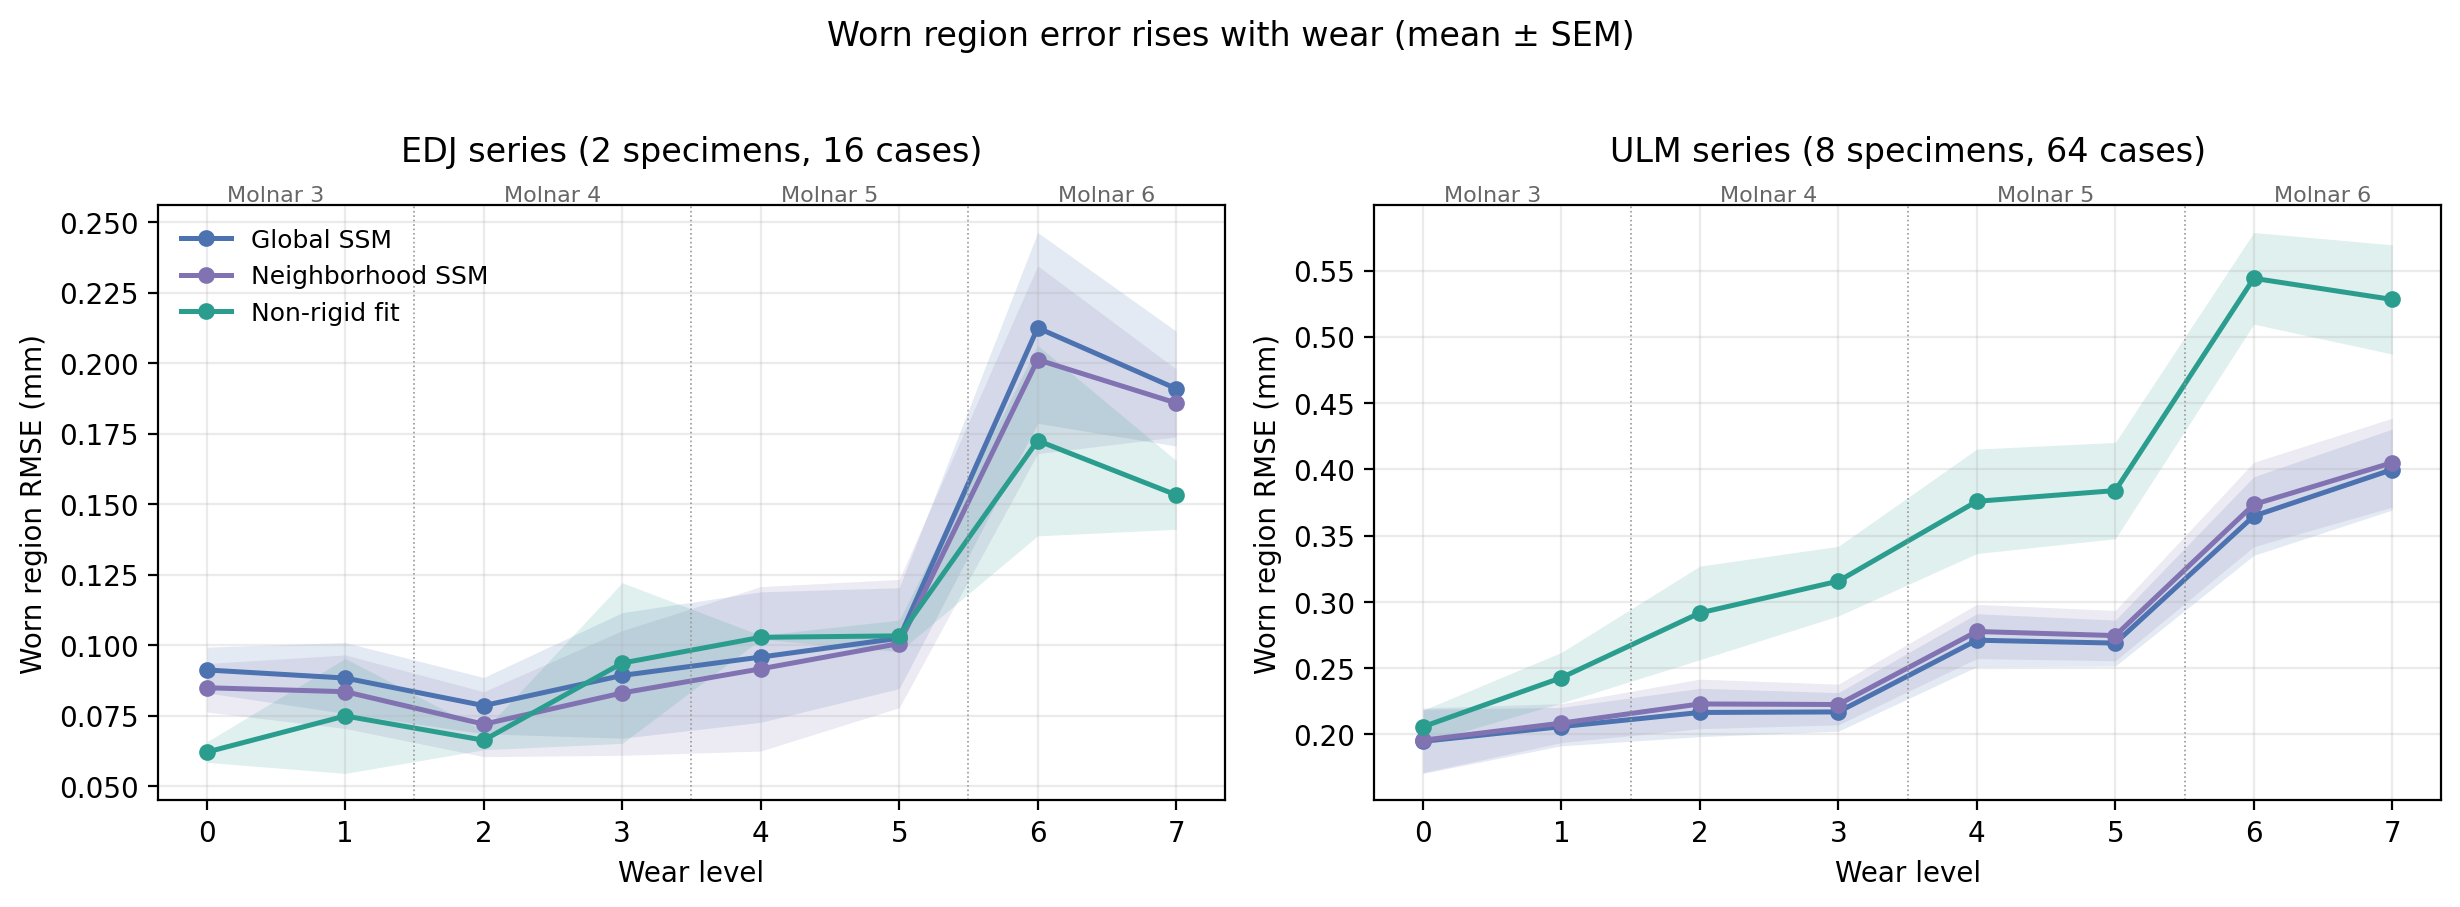
\includegraphics[width=\textwidth]{fig_error_vs_wear.png}
\caption{Worn-region RMSE against wear level. Left, EDJ series (2 specimens,
  16 cases, $100{,}000$ points per tooth); right, ULM series (8 held-out
  specimens, 64 cases, $10{,}000$ points per tooth). Points are means over the
  cases at each level and shaded bands are $\pm1$ standard error of the mean; on
  the EDJ series each point rests on only two cases. Dotted lines separate Molnar
  stages 3 to 6. The Global and Neighborhood SSM curves nearly overlap on both
  series. On the ULM series the non-rigid fit has the highest error at every
  level, and the gap opens from L2 onward; on the EDJ series it has the lowest
  error at light wear (L0 to L2) and at Molnar stage~6, and the three methods
  are close in between.}
\label{fig:wear}
\end{figure*}

\subsection{Reading the primary layer}
\label{sec:primary}

The two series rank the methods in opposite orders.

On the densely sampled EDJ series the non-rigid fit restores worn anatomy best,
at $0.104\mm$ against $0.113\mm$ for Neighborhood SSM and $0.119\mm$ for Global
SSM. It beats Global SSM in 12 of the 16 cases, a 13\% reduction in error
(Wilcoxon signed-rank test, $p=0.025$). With only two specimens, however, this
series cannot show that the ranking holds across teeth.

On the held-out ULM series, sampled at a tenth of that density, the order is
reversed. Global SSM restores worn anatomy best, at $0.267\mm$, Neighborhood SSM
is close behind at $0.273\mm$, and the non-rigid fit is worst at $0.361\mm$,
35\% above Global SSM. The non-rigid fit has the lower error in only 5 of 64
cases and for none of the eight specimens; a bootstrap that resamples specimens
puts its excess error between $0.063$ and $0.122\mm$ (Wilcoxon signed-rank test
over specimens, $p=0.008$). Section~\ref{sec:density} traces the difference to the
way the non-rigid warp behaves at low point density.

\subsection{Reading the secondary and tertiary layers}
\label{sec:secondary}

The non-rigid fit leads both supporting layers on both series. Its full-surface
Chamfer distance is 58\% below Global SSM on the EDJ series ($0.022$ against
$0.054\mm$) and 43\% below on the ULM series ($0.069$ against $0.120\mm$), and its
distance to the worn scan is roughly half that of either shape model. This is what
its design predicts: it is optimised to hug the observed scan, so on any metric
that rewards agreement with intact surface it will lead by construction.

The ULM series shows why the layers must be kept apart. There the non-rigid fit
has the best full-surface Chamfer distance of the three methods and the worst
worn-region error. A whole-surface score would rank it first; the question that
matters, whether the missing anatomy came back, ranks it last. Comparing the same
metric across layers makes the same point: worn-region RMSE is 3.0 times
full-surface RMSE for the non-rigid fit on the EDJ series and 2.25 times on the
ULM series, against 1.6 to 1.7 times for the shape models on both.

\subsection{The two SSM variants}

Global and Neighborhood SSM produce nearly the same numbers, and the two series
lean in opposite directions. On the EDJ series Neighborhood SSM has the lower
worn-region error in 13 of 16 cases, a 4.9\% reduction (Wilcoxon signed-rank
test, $p<0.001$), but that series has only two specimens. On the held-out ULM
series it has the higher error: 1.9\% above Global SSM, lower in only 14 of 64
cases and for one of eight specimens ($p=0.016$ over specimens; a bootstrap that
resamples specimens gives a 95\% interval of $0.003$ to $0.008\mm$ for the excess).
In shape space the two are equally close (\S\ref{sec:shaperesults}). The
neighborhood model therefore shows no consistent gain. \S\ref{sec:tie} examines
why.

\begin{figure*}[!t]
\centering
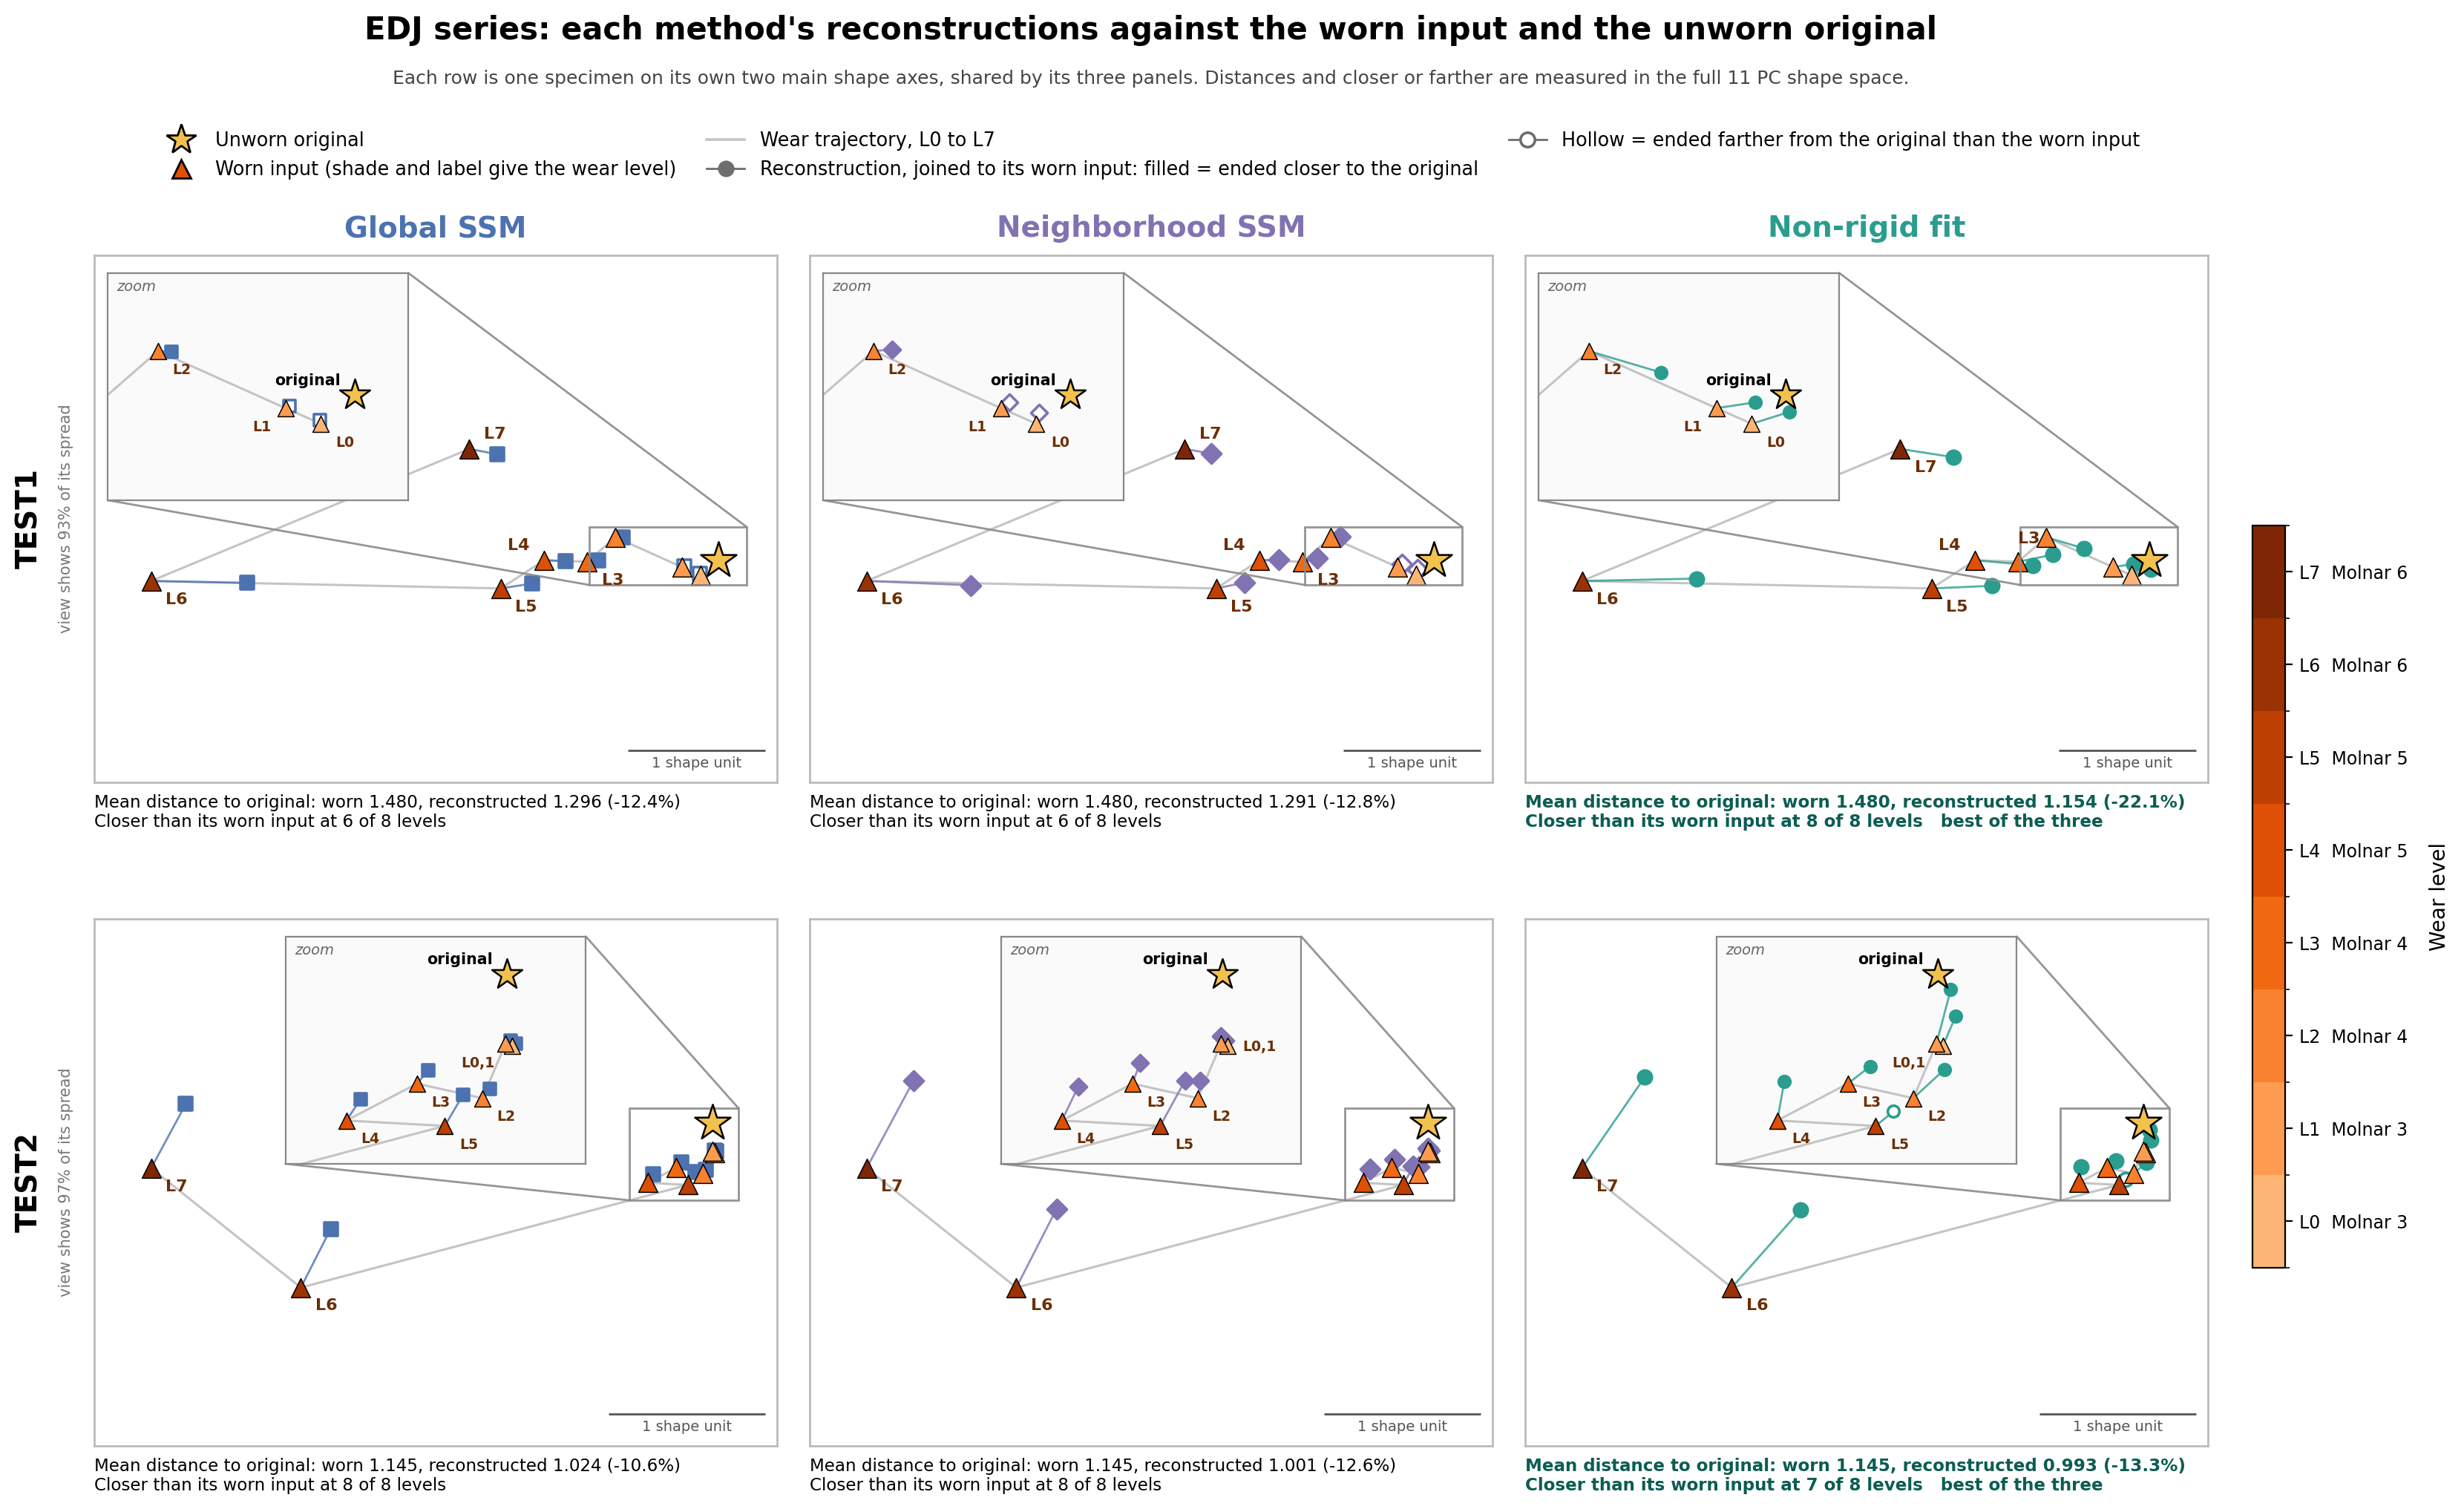
\includegraphics[width=\textwidth]{fig_shape_methods_edj.png}
\caption{Where each reconstruction lands in shape space, EDJ series. Rows are
  the two test specimens and columns the three methods. Each row is drawn on the
  two principal axes of that specimen's own points, shared by its three panels so
  that they can be compared directly; these axes capture 93\% (TEST1) and 97\%
  (TEST2) of the spread. Triangles are the worn inputs, shaded and labelled by
  wear level (the colour bar gives the Molnar stage) and joined in order of wear
  by the grey line. The star is the unworn original. Each reconstruction is
  joined to the worn input it was built from and is drawn filled if it ended
  closer to the original than that input, or hollow if it ended farther away.
  Insets enlarge the light-wear cases crowded near the original. Distances, and
  the filled or hollow decision, use the full 11-component shape space
  (\S\ref{sec:shapespace}) and are in Procrustes shape units. The text under each
  panel gives the mean distance to the original for the worn inputs and for the
  reconstructions, and the number of levels at which the reconstruction moved
  closer; the best of the three methods in each row is shown in green.}
\label{fig:shape_edj}
\end{figure*}

\subsection{Behaviour with increasing wear}
\label{sec:wear}

Error rises with wear for every method on both series (Figure~\ref{fig:wear},
Table~\ref{tab:levels}), which is the expected pattern: more missing anatomy means
more to invent and less evidence to invent it from. The rank correlation between
worn-region RMSE and wear level is $\rho = 0.65$ to $0.86$ on the EDJ series
($p \le 0.006$) and $0.73$ to $0.80$ on the ULM series ($p<0.001$).

The rise is uneven. At light wear the EDJ shape models are nearly flat, and even
dip at L2, because the worn region there is tiny (0.6 to 2.9\% of the crown) and
the error is dominated by how well the model matches the specimen as a whole.
Between L5 and L6, the transition into Molnar stage~6, error jumps on both series:
it roughly doubles on the EDJ series ($0.102 \to 0.212\mm$ for Global SSM) and
rises by a third on the ULM series ($0.269 \to 0.365\mm$). On the EDJ series it
eases again at L7 for every method, a level that rests on only two cases. This jump, rather than
the gradual rise below it, is the practically important feature of these results,
and \S\ref{sec:severe} discusses it.

The relative standing of the non-rigid fit also depends on wear. On the ULM series
it is 12\% above Global SSM at Molnar stage~3 and about 40\% above at stages 4, 5
and 6: its disadvantage grows as soon as there are cusps to rebuild. On the EDJ
series it is 24\% below Global SSM at stage~3, within 5\% at stages 4 and 5, and
19\% below at stage~6.

\subsection{Recovery in shape space}
\label{sec:shaperesults}

Figure~\ref{fig:shape_edj} shows where each EDJ reconstruction lands relative to
its worn input and its original. Figures~\ref{fig:shape_ulm1}
and~\ref{fig:shape_ulm2} in the supplementary material show the same for the ULM
series, and Figures~\ref{fig:overview_edj} and~\ref{fig:overview_ulm} place the
test specimens among the training teeth.

\paragraph{The shape models move reconstructions toward the original.}
On the EDJ series all three methods bring overall shape closer to the original in
14 or 15 of 16 cases. The average distance to the original falls from 1.31 for the
worn inputs to 1.16 (Global SSM), 1.15 (Neighborhood SSM) and 1.07 (non-rigid
fit); the non-rigid fit moves closest on both specimens. On the ULM series Global
and Neighborhood SSM move closer in 57 and 55 of 64 cases, but by little: the
average distance falls from 1.41 to 1.37 and 1.38. Even at L0 the worn inputs sit
away from their originals (mean distance 0.27 on the EDJ series and 0.59 on the
ULM series), reflecting both the wear already present at Molnar stage~3 and
differences in how separately corresponded scans sample the same surface.

\paragraph{On the ULM series the non-rigid fit moves away.}
The non-rigid fit ends closer to the original than its worn input in only 10 of
64 ULM cases, and its average distance rises from 1.41 to 1.48; it ends farther
away on average for every one of the eight specimens. This matches its worn-region
error: the warp that pulls the reconstruction onto the scan also pulls part of the
rebuilt anatomy back toward the worn shape (\S\ref{sec:density}).

Taken together, the surface metrics and the shape-space distances agree on the
ranking within each series. They also show how modest the recovery of overall
shape is on the ULM series, where the best method reduces the distance to the
original by only 3\% on average.

\begin{figure*}[!t]
\centering
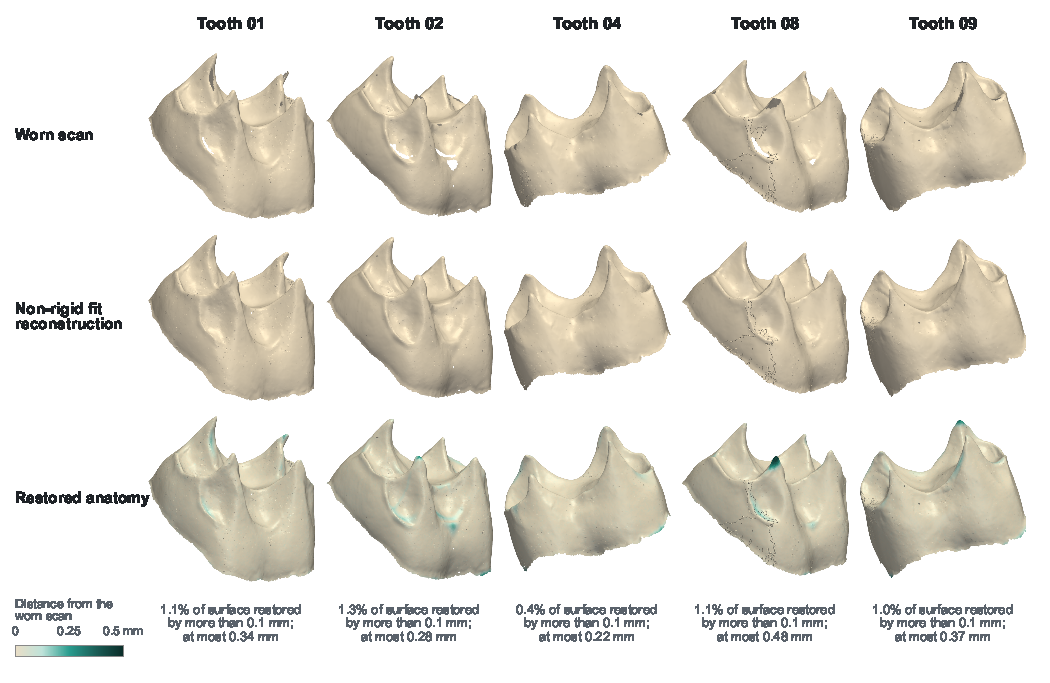
\includegraphics[width=\textwidth]{fig_realworn.pdf}
\caption{Non-rigid fit reconstructions of five naturally worn EDJ surfaces, for
  which no unworn original exists. Columns are the five teeth that passed the
  registration check (\S\ref{sec:regcheck}); all three views of a tooth share one
  camera, with the occlusal side up. \textbf{Top:} the worn scan, drawn as the part
  of the reconstructed surface that lies within $0.1\mm$ of the scanned points, so
  that gaps in the scan appear as openings. \textbf{Middle:} the reconstruction.
  \textbf{Bottom:} the reconstruction coloured by its distance from the worn scan,
  which marks the anatomy the reconstruction adds. The figures under each column
  give the share of reconstructed points that lie more than $0.1\mm$ from the
  scan and the largest such distance. The additions sit at dentine horn tips
  breached by wear, in holes in the scans themselves, and in places along the
  cervical margin.}
\label{fig:realworn}
\end{figure*}

\subsection{Naturally worn teeth}
\label{sec:natural}

Figure~\ref{fig:realworn} shows the non-rigid fit applied to five naturally worn
EDJ surfaces, reconstructed with the same 17-tooth model. With no original to
compare against, these cases show what the method does rather than how accurate it
is. It leaves the scanned surface in place and adds anatomy only where the scan
has none: between 0.4 and 1.3\% of the reconstructed surface lies more than
$0.1\mm$ from the worn scan, and no point lies more than $0.48\mm$ from it. The
additions sit at dentine horn tips where wear has breached the junction and in
holes in the scans. Their small size also shows that these specimens are only
lightly worn at the level of the enamel dentine junction; the artificially worn
series, which reach Molnar stage~6, remain the only test of heavier wear.
% ===========================================================================
\section{Discussion}
\label{sec:discussion}
% ===========================================================================

\subsection{What the numbers mean physically}

A ULM3 EDJ surface spans roughly $7$ to $9\mm$ in its largest dimension. A
worn-region RMSE of $0.10$ to $0.12\mm$ on the EDJ series is therefore on the order
of $1.2$ to $1.5\%$ of crown dimension, and $0.27\mm$ on the ULM series about $3$ to
$4\%$: the reconstructed cusp sits one to three tenths of a millimetre from where
it originally was.

Whether that is good enough depends entirely on the question being asked. For
cusp-tip position, occlusal basin depth, relative cusp height or crown height,
which are measured in whole millimetres and compared across specimens that
differ by more than that, errors of this size are comfortably inside tolerance.
For fine surface texture they are not: crenulation, secondary ridging and the
fine relief of the occlusal basin have amplitudes comparable to the error itself,
so a reconstruction cannot be used to score those features. A practical rule is
that the reconstruction is trustworthy for measurements whose expected
between-specimen differences exceed roughly $0.5\mm$, and not otherwise.

The gap between the primary and secondary layers deserves emphasis. On the ULM
series the non-rigid fit has the best whole-surface Chamfer distance
($0.069\mm$) and the worst worn-region error ($0.361\mm$). Reporting only
whole-surface Chamfer, as is common in this literature, would have ranked it
first of the three methods, although it restores worn anatomy worst. The
difference between the two layers \emph{is} the difference between reproducing
a tooth and restoring one: the whole-surface figure is dominated by intact enamel
the method essentially copied from its input.

\subsection{Why the non-rigid fit depends on point density}
\label{sec:density}

The non-rigid fit is designed to leave the worn region alone. Points far from the
scan receive no confidence, so they should keep the shape model's anatomy while
the rest of the reconstruction is pulled onto the scan. In practice the
thin-plate-spline warp is smooth, so it carries part of the pull from nearby
confident points into the region that has no scan support.

How far that happens depends on how the confidence band is set. The band is
defined in multiples of the median point spacing, starting at eight spacings and
narrowing to three. At $10{,}000$ points per tooth the spacing is about $0.06\mm$,
so the band starts near $0.5\mm$, wide enough to reach from the edge of a wear
facet onto the cusps that need rebuilding. At $100{,}000$ points it is about
$0.13\mm$. The consequence is measurable. On the ULM series, points the fit itself
marks as unsupported (confidence below 0.2) move $0.38\mm$ on average during the
warp, with a net downward shift of $0.11\mm$, more than twice as far as the
confident points ($0.17\mm$). On the EDJ series the same points move only
$0.10\mm$, with no systematic downward shift. The rebuilt cusps are therefore
partly flattened back toward the worn surface at low density and largely
preserved at high density, which matches the opposite rankings in
Table~\ref{tab:main} and the growth of the non-rigid fit's disadvantage from
Molnar stage~4 onward on the ULM series.

Two fixes follow directly, neither of which we have tested: define the confidence
band in millimetres rather than in point spacings, or exclude the estimated
missing region (\S\ref{sec:global}) from the warp altogether. Until one of them is
validated, the non-rigid fit should be used only on densely sampled teeth, and the
global shape model is the better choice at $10{,}000$ points. Because the
parameters of the non-rigid fit were fixed before the corrected evaluation, we have
not tuned them on these results.

\subsection{Comparison with statistical shape work on teeth}
\label{sec:compare}

Our figures fall inside the band the dental SSM literature reports
(Table~\ref{tab:lit}), which is the appropriate sanity check for a new pipeline:
not that it beats prior work, but that it lands in the right regime.

\begin{table*}[!t]
\centering
\caption{Reported reconstruction error across the literature. Most prior studies
  report error over the \emph{whole} reconstructed surface, so the comparable
  figure from this work is the secondary layer, not the primary. Ranges span the
  three methods.}
\label{tab:lit}
\small
\begin{tabularx}{\textwidth}{@{}>{\raggedright\arraybackslash}p{3.4cm}>{\raggedright\arraybackslash}p{4.2cm}LL@{}}
\toprule
\textbf{Study} & \textbf{Material} & \textbf{Task} & \textbf{Reported error} \\
\midrule
\citet{buchaillard2007tooth} & human teeth & SSM surface reconstruction & $<0.2\mm$ (5 PCs); $<0.1\mm$ (13 PCs) \\
\citet{woods2017ssm} & 27 mandibular canines, archaeological & SSM reconstruction & $<0.2\mm$ (5 PCs), ${\approx}0.7\%$ of crown length \\
\midrule
\textbf{This work (EDJ)} & primate ULM3 EDJ & worn-region restoration & $\mathbf{0.104}$--$\mathbf{0.119\mm}$ RMSE \\
\textbf{This work (EDJ)} & primate ULM3 EDJ & full surface (secondary) & $\mathbf{0.022}$--$\mathbf{0.054\mm}$ Chamfer \\
\textbf{This work (ULM)} & primate ULM3 EDJ, held out & worn-region restoration & $\mathbf{0.267}$--$\mathbf{0.361\mm}$ RMSE \\
\textbf{This work (ULM)} & primate ULM3 EDJ, held out & full surface (secondary) & $\mathbf{0.069}$--$\mathbf{0.120\mm}$ Chamfer \\
\bottomrule
\end{tabularx}
\end{table*}

Two qualifications govern how that table should be read. First, most prior
studies report error over the \emph{whole} reconstructed surface, so the rows
comparable to their numbers are our secondary layer ($0.022$ to $0.054\mm$
Chamfer on the EDJ series and $0.069$ to $0.120\mm$ on the ULM series), not our
primary. On that comparison our figures are below the $<0.2\mm$ those studies
report, but that is not a claim of superiority, because of the second
qualification. They reconstruct from complete or lightly damaged inputs, largely
testing how well a shape model can represent a tooth it has effectively seen,
whereas the present task withholds a genuinely missing region and asks the model
to invent it. The two tasks are different in kind, and the table establishes
regime agreement rather than a ranking.

Against the anthropological baselines no numeric comparison is possible at all,
because Profile, Polynomial and Pen Tool return scalar measurements rather than
surfaces and are validated on different quantities
\citep{ohara2022reconstructing}. The relevant claim is one of scope: those
methods are reported reliable only for lightly worn crowns, whereas this pipeline
returns a complete surface across Molnar stages 3 to 6 with a quantified error that
rises predictably with wear, so a user can decide, from the wear stage alone,
whether the reconstruction is accurate enough for their question.

\subsection{Why image-based methods are not comparable}
\label{sec:imagebased}

Published 3D dental reconstruction from photographs or radiographs reports
Chamfer distances an order of magnitude larger than ours, and it would be easy to
present that as a favourable comparison. It is not one. The gap reflects problem
difficulty, not method quality. TeethDreamer \citep{teethdreamer2024} infers 3D
geometry from five 2D photographs; Occudent \citep{occudent2023} works from a
single panoramic radiograph. Both must recover depth, absolute scale and tooth
identity from projections that discard exactly that information, a severely
ill-posed problem. Our input is already a metric 3D surface in millimetres, and
only a bounded region of it is missing. Tabulating the two side by side would
mislead a reader about what has been achieved, so we do not do so.

\subsection{Why the neighborhood model gains nothing consistent}
\label{sec:tie}

The neighborhood model was motivated by the expectation that a locally fitted
prior would beat a population prior. It does not do so consistently. It is 4.7\%
better than the global model on the two-specimen EDJ series and 1.9\% worse on the
eight held-out ULM specimens, and both differences are far below anything that
would matter for measurement.

Two explanations fit the data. The first is that the adaptive threshold is
generous relative to the spread of the training sample. If most specimens fall
within $\mathrm{median} + 2\,\mathrm{IQR}$ of the query tooth, then most
selections return the full neighbour quota, and the local model is built from
the teeth that happen to be nearest rather than from a genuinely distinct
subgroup. The second is that the trade the method makes is simply not favourable
here: a $K$-neighbour model retains at most $K-1$ modes, so whatever is gained
from a more relevant mean is given back in reduced expressive range. The loss is
severe: with $K=5$ on the EDJ series and $K=10$ on the ULM series the local model
keeps at most 4 or 9 modes, against 14 and 30 in the global models.

These are distinguishable by experiment. A sweep over the threshold multiplier and
the neighbour cap would show whether tightening selection produces a genuinely
local prior and whether that prior helps, but we have not run it. Until then the
global model is the better default: it is simpler and at least as accurate on the
held-out series.

\subsection{Failure at severe wear}
\label{sec:severe}

All methods degrade sharply at Molnar stage~6. Between level~5 and level~6
worn-region RMSE roughly doubles on the EDJ series ($0.102 \to 0.212\mm$ for
Global SSM) and rises by a third on the ULM series ($0.269 \to 0.365\mm$), a jump
rather than a continuation of the gradual rise below it.

The mechanism is straightforward and worth stating plainly. As wear removes more
of the crown, two things happen at once: the fit is constrained by fewer
surviving points, and it is asked to invent more geometry. Both push the solution
toward the model mean, because with weak evidence the regularisation term in
Equation~\eqref{eq:fit} dominates and the coefficients shrink toward zero. The
reconstruction becomes an average tooth wearing the observed tooth's remaining
surface, and that is precisely the point at which it stops being evidence about
this specimen and starts being evidence about the training sample.

The non-rigid fit behaves differently on the two series here too. On the dense
EDJ series it is the best of the three at stage~6 ($0.163\mm$ against $0.202\mm$
for Global SSM), because the confident scan points it relies on still pin the
intact rim in place. On the sparse ULM series it is the worst ($0.536\mm$ against
$0.382\mm$), because stage~6 has the largest unsupported region for its warp to
distort (\S\ref{sec:density}).

\paragraph{Practical guidance.}
Through Molnar stage~5, reconstructions from densely sampled teeth are accurate to
roughly $0.1\mm$, and those from teeth sampled at $10{,}000$ points to roughly
$0.2$ to $0.27\mm$ with the global shape model; both are suitable for
cusp-position and crown-height work. At stage~6 reconstructions should be treated
as indicative only (useful for visualisation or for establishing that a specimen
is broadly consistent with a group, but not for measurement) and always reported
with the error figures above attached. At low point density the non-rigid fit
should not be used until its warp is constrained (\S\ref{sec:density}). We would
not recommend using these reconstructions to score discrete traits at any wear
stage, since trait expression depends on fine relief the method does not recover.

% ===========================================================================
\section{Limitations}
\label{sec:limitations}
% ===========================================================================

\begin{enumerate}
  \item \textbf{Artificial wear is not natural wear.} Our series are produced by
        progressive digital removal from a known original. Natural attrition
        differs in ways that probably matter: it involves dentine exposure with
        differential wear rates between enamel and the softer dentine, secondary
        dentine deposition as the pulp responds, and wear facets whose
        orientation is determined by occlusion rather than by a uniform
        subtraction. Digital wear also leaves a cleaner boundary than attrition
        does. The error figures here should therefore be read as a lower bound on
        what to expect from natural specimens.
  \item \textbf{Single tooth position, single broad taxon.} Everything reported
        is ULM3. Third molars are the most morphologically variable position in
        the molar row, so a model trained on them may generalise poorly to M1 or
        M2, and we have not tested other positions or other taxa.
  \item \textbf{Training sample size.} The EDJ model is built from 17 specimens
        and retains 14 modes, close to the ceiling of $n-1$ modes a sample of
        that size can support. Shape models on small samples risk
        under-representing rare morphology, and a specimen unlike anything in the
        training set will be reconstructed toward what the model has seen. The
        90-specimen ULM model is more comfortable in this respect, and the
        difference between the two is a plausible contributor to their differing
        error levels.
  \item \textbf{Two sampling densities, two specimens.} The two series were
        corresponded at different densities ($100{,}000$ versus $10{,}000$ points
        per tooth). Density changes every nearest-neighbour metric and, as
        \S\ref{sec:density} shows, the behaviour of the non-rigid fit, so the EDJ
        and ULM panels of Table~\ref{tab:main} should be read independently. The
        EDJ series also has only two specimens, so its ranking of the methods
        cannot be shown to hold across teeth. The worn EDJ meshes available to us
        were truncated files; the EDJ wear mask therefore uses the
        $100{,}000$-point samples taken from the intact meshes in Stage~1, which
        the mask rule is designed to accept (\S\ref{sec:protocol}).
  \item \textbf{No inter-operator baseline.} We have not compared against manual
        reconstruction by an experienced observer. That comparison would be the
        most meaningful anthropological reference point, since the practical
        question is not whether the method is accurate in the abstract but
        whether it is at least as good as, and more reproducible than, what a
        trained person would do by hand.
  \item \textbf{The missing-region estimate uses a fixed fraction.} The worn
        region is estimated by treating a fixed 15\% of points as missing
        (\S\ref{sec:global}). The actual worn share ranges from under 1\% to
        about 25\% of the crown, so at light wear most selected points are in
        fact intact, and at severe wear some worn anatomy is treated as observed.
        A fraction that adapts to each specimen's wear is the most obvious
        target for improvement.
  \item \textbf{The non-rigid fit was not tuned for density.} Its parameters
        were fixed before the corrected evaluation and are defined relative to
        point spacing. We identify the likely remedy (\S\ref{sec:density}) but
        have not tested it, so its ULM results describe the method as
        configured, not as it could be.
\end{enumerate}
% ===========================================================================
\section{Toward a reconstruction library}
\label{sec:library}
% ===========================================================================

The pipeline is being packaged as a library, so that this style of reconstruction
is available to researchers as a set of composable, documented steps rather than
a monolithic script. The motivation is not convenience but validity: no single
configuration is right for all material. Sample size, scan resolution, wear
severity and the morphological question all change what the appropriate settings
are, and a tool that hides those choices behind defaults will silently produce
inappropriate reconstructions for material unlike the one it was tuned on. The
library's purpose is to make every such choice explicit, documented and
adjustable.

\subsection{Design principles}

\begin{itemize}
  \item \textbf{Stages are independent.} Correspondence, reconstruction and
        evaluation communicate through files on disk rather than through shared
        state. A researcher with their own correspondence method, or their own
        preferred evaluation, can substitute it and keep the rest.
  \item \textbf{Every choice is a named parameter} with a documented default and
        a stated effect (Table~\ref{tab:params}). Nothing consequential is a
        hard-coded constant.
  \item \textbf{Reconstruction strategies are interchangeable} behind one
        interface, so adding a fourth does not disturb the first three and any
        new method is automatically comparable to them under the same protocol.
  \item \textbf{Evaluation is separable from reconstruction.} The scoring code
        shares no state with the methods it scores, so results cannot be produced
        by a metric that has been tuned, however inadvertently, to a particular
        method.
\end{itemize}

\subsection{Choosing parameters}

Table~\ref{tab:params} lists every exposed parameter. Three deserve particular
attention from anyone adopting the pipeline.

\code{proxy\_missing\_fraction} is the most consequential. It sets how much of
the crown is assumed to be worn away when the worn region is not known
independently. Set too high, healthy anatomy is discarded and replaced with model
estimate, and the reconstruction is worse than the input in regions that needed
no repair; set too low, genuinely worn anatomy is treated as observed and drags
the fit down toward the worn surface. Because appropriate values scale with wear
severity, a single value across a mixed-wear assemblage is a compromise, and
stratifying by wear stage is worth the effort.

\code{regularization} ($\lambda$) controls how strongly the shape prior is
enforced. Raise it when little of the tooth survives, since with weak evidence an
unconstrained fit will produce implausible geometry; lower it for lightly worn,
well-sampled teeth, where the data can be trusted to speak for itself.

\code{n\_points} governs the resolution of the whole analysis. It should be set
from the resolution of the input meshes, not from the desired output: sampling
$100{,}000$ points from a mesh with $3{,}000$ vertices adds no information and
costs correspondence time proportional to the square of the count.

\subsection{Intended workflow}

A researcher supplies a directory of unworn reference teeth and a directory of
worn specimens, chooses a reconstruction strategy, and receives reconstructed
surfaces in the original millimetre coordinate frame together with a per-specimen
evaluation record. Where ground truth is available the evaluation reports the
full three-layer protocol of \S\ref{sec:protocol}. Where it is not, which is
the normal case for real material, the evaluation stage still reports the
diagnostics needed to judge whether a reconstruction should be trusted: the
residual of the model fit at observed points, the fitted coefficients and how far
each sits from the training mean in standard deviations, and the fraction of
surface that was treated as missing. A reconstruction whose coefficients sit near
the $\pm4\sigma$ clipping bound, or whose missing fraction is far from what the
specimen's wear stage would suggest, should be inspected before use.

\begin{table*}[!t]
\centering
\caption{Parameters exposed at each pipeline stage, with defaults and the
  circumstances that warrant changing them.}
\label{tab:params}
\footnotesize
\begin{tabularx}{\textwidth}{@{}>{\raggedright\arraybackslash}p{4.0cm}>{\raggedright\arraybackslash}p{1.8cm}LL@{}}
\toprule
\textbf{Parameter} & \textbf{Default} & \textbf{Controls} & \textbf{When to change it} \\
\midrule
\multicolumn{4}{@{}l}{\itshape Stage 1: correspondence} \\
\code{n\_points}          & 20{,}000  & points sampled per tooth & raise to 100k for fine detail; match to input mesh resolution, not desired output \\
\code{registration\_mode} & direct    & CPD on all points, or coarse-to-fine & use coarse-to-fine above ${\sim}50$k points, where CPD cost becomes prohibitive \\
\code{cpd\_points}        & 43{,}000  & points used for CPD in coarse-to-fine & trade registration accuracy against memory \\
\code{displacement\_knn}  & 3         & neighbours for upsampling the deformation & raise to smooth a noisy displacement field \\
\code{auto\_template}     & off       & pick the most central specimen as template & leave on unless a specific reference specimen is required \\
\code{scale\_method}      & bbox diag & how size is removed & switch to unit sphere if bounding boxes are unstable across specimens \\
\code{seed}               & 42        & sampling reproducibility & fix for publication runs so results are exactly reproducible \\
\addlinespace[2pt]
\multicolumn{4}{@{}l}{\itshape Stages 2a and 2b: shape model reconstruction} \\
\code{variance\_threshold} & 0.99 & how many PCA modes to keep & lower (0.90 to 0.95) for small or noisy training samples, where late modes encode noise \\
\code{n\_components}       & auto & explicit mode count & set directly for a controlled ablation over model complexity \\
\code{regularization} ($\lambda$) & 1.0 & strength of the shape prior & raise when little of the tooth survives; lower for lightly worn, well-sampled teeth \\
\code{proxy\_missing\_fraction} & 0.15 & fraction treated as missing when the worn region is unknown & \textbf{the most consequential parameter}: too high overwrites healthy anatomy, too low leaves wear unrepaired; stratify by wear stage where possible \\
\code{proxy\_mask\_method} & scan-distance & how the missing region is estimated (\S\ref{sec:global}) & keep the default; \code{mean} reproduces the earlier mean-shape heuristic for comparison only \\
\code{max\_neighbors} ($K$) & 5   & cap on neighbours for the local model & raise with a larger training pool; note the model retains at most $K-1$ modes \\
\code{threshold\_iqr\_mult} & 2.0 & how permissive neighbour selection is & lower it to make selection genuinely selective (\S\ref{sec:tie}) \\
\code{ssm\_variance}        & 0.95 & variance retained by the local model & as above \\
\addlinespace[2pt]
\multicolumn{4}{@{}l}{\itshape Stage 2c: non-rigid fit} \\
\code{iters} & 12  & coarse-to-fine rounds & raise for large initial misalignment \\
\code{step}  & 0.6 & how far to move per round & lower for stability, raise for speed \\
\code{far\_start} / \code{far\_end} & 8 / 3 & the confidence band, in median spacings & keep the band below about $0.15\mm$; at $10{,}000$ points the default reaches $0.5\mm$ and flattens rebuilt cusps (\S\ref{sec:density}) \\
\code{smooth\_start} / \code{smooth\_end} & 1.2 / 0.3 & warp smoothness, annealed across iterations & raise to prevent local distortion on sparse landmark sets \\
\code{tight\_snap} & 0 & final snap of confident points onto the scan & leave at 0; positive values cause points to clump many-to-one on scan vertices \\
\addlinespace[2pt]
\multicolumn{4}{@{}l}{\itshape Stage 3: evaluation and surface output} \\
\code{wear\_mult}        & 2.0 & wear-mask threshold, in spacings of the original, plus 1.5 spacings of the worn-surface sample & raise for noisy scans so that noise is not flagged as wear \\
\code{n\_gt}             & 120{,}000 & sampling density of the reference surface & keep matched to the reconstruction's density, or nearest-neighbour metrics are biased \\
ICP mode                 & point-to-plane & registration before measuring & match whatever the comparison literature used, so numbers are comparable \\
\code{poisson\_depth}    & auto & octree depth for meshing & lower for sparse clouds, where deep octrees produce artefacts \\
\code{density\_quantile} & 0.01 & fraction of low-density fringe trimmed & raise to trim more of the extrapolated boundary Poisson produces \\
\code{smooth\_iter}      & 30 & Taubin smoothing passes & lower to preserve fine relief \\
\bottomrule
\end{tabularx}
\end{table*}

% ===========================================================================
\section{Conclusion}
\label{sec:conclusion}
% ===========================================================================

We have presented a landmark-free pipeline that reconstructs pre-wear EDJ
surfaces of primate ULM3s from worn 3D scans, and evaluated it against known
ground truth across Molnar wear stages 3 to 6 on two independent series.
Worn-region restoration error is $0.104$ to $0.119\mm$ on the densely sampled
16-case EDJ series and $0.267$ to $0.361\mm$ on the 64-case held-out ULM series,
within the band reported for statistical shape reconstruction of teeth elsewhere
and obtained without manual landmarking at any stage. Which method is best depends
on point density. On the dense series the non-rigid fit restores worn anatomy
best; on the held-out series, sampled at a tenth of that density, the global shape
model does, and the non-rigid fit is 35\% worse because its warp pulls the rebuilt
cusps back toward the worn surface, even though it matches the intact surface
most closely. The neighborhood model gives no consistent gain over the global one.
All methods degrade sharply at Molnar stage~6, and we regard that as the practical
limit of the approach as it stands.

The broader contribution is methodological, and this study illustrates it twice.
Because a worn tooth is mostly intact, any aggregate surface metric is dominated
by the part of the problem that was never hard, and a method that changes nothing
at all can post excellent numbers. On the held-out series that inflation would
have ranked the non-rigid fit first. The wear mask itself must also be robust to
sampling: a mask computed against a sparse sample of the worn scan flags intact
surface as worn, and in our first analysis it covered about 80\% of the crown
instead of about 12\%, hiding the difference between the methods. Registration
needs the same scrutiny, since a tooth registered half a turn out still yields a
smooth, plausible cloud. By scoring restoration on a shared, method-agnostic mask of the anatomy
wear actually removed, and reporting whole-surface agreement only as supporting
evidence explicitly excluded from the ranking, we avoid that inflation. We
recommend the same separation for future work in this area, and note that the
three-layer structure is not specific to teeth: it applies wherever a method is
asked to complete a partially observed shape.

\section*{Data and code availability}

The reconstruction pipeline, evaluation protocol and per-case results are
available in the project repository; \code{ssm\_pipeline/run\_fixed\_pipeline.sh}
reproduces every reported result from the corrected Stage~1 outputs. Per-case numbers behind every table in
\S\ref{sec:results} are in the evaluation CSV files produced by
\code{evaluate\_paper\_protocol.py}. The figures, the per-stage and paired
statistics and the shape-space analysis are produced from those files and the
corresponded point clouds by \code{data\_analysis/benchmark\_analysis.py}.

% Flush any pending floats so no table is stranded after the references.
\clearpage

{\footnotesize
\bibliography{references}
}

% ===========================================================================
% SUPPLEMENTARY MATERIAL
% ===========================================================================
\clearpage
\onecolumn
\setcounter{figure}{0}
\renewcommand{\thefigure}{S\arabic{figure}}

\section*{Supplementary material}

These figures extend the shape-space analysis of \S\ref{sec:shaperesults}.
Figures~\ref{fig:shape_ulm1} and~\ref{fig:shape_ulm2} show the ULM series in the
same layout as Figure~\ref{fig:shape_edj}. Figures~\ref{fig:overview_edj}
and~\ref{fig:overview_ulm} place the test specimens of each series among the
unworn training teeth that define its shape space.

\begin{figure}[H]
\centering
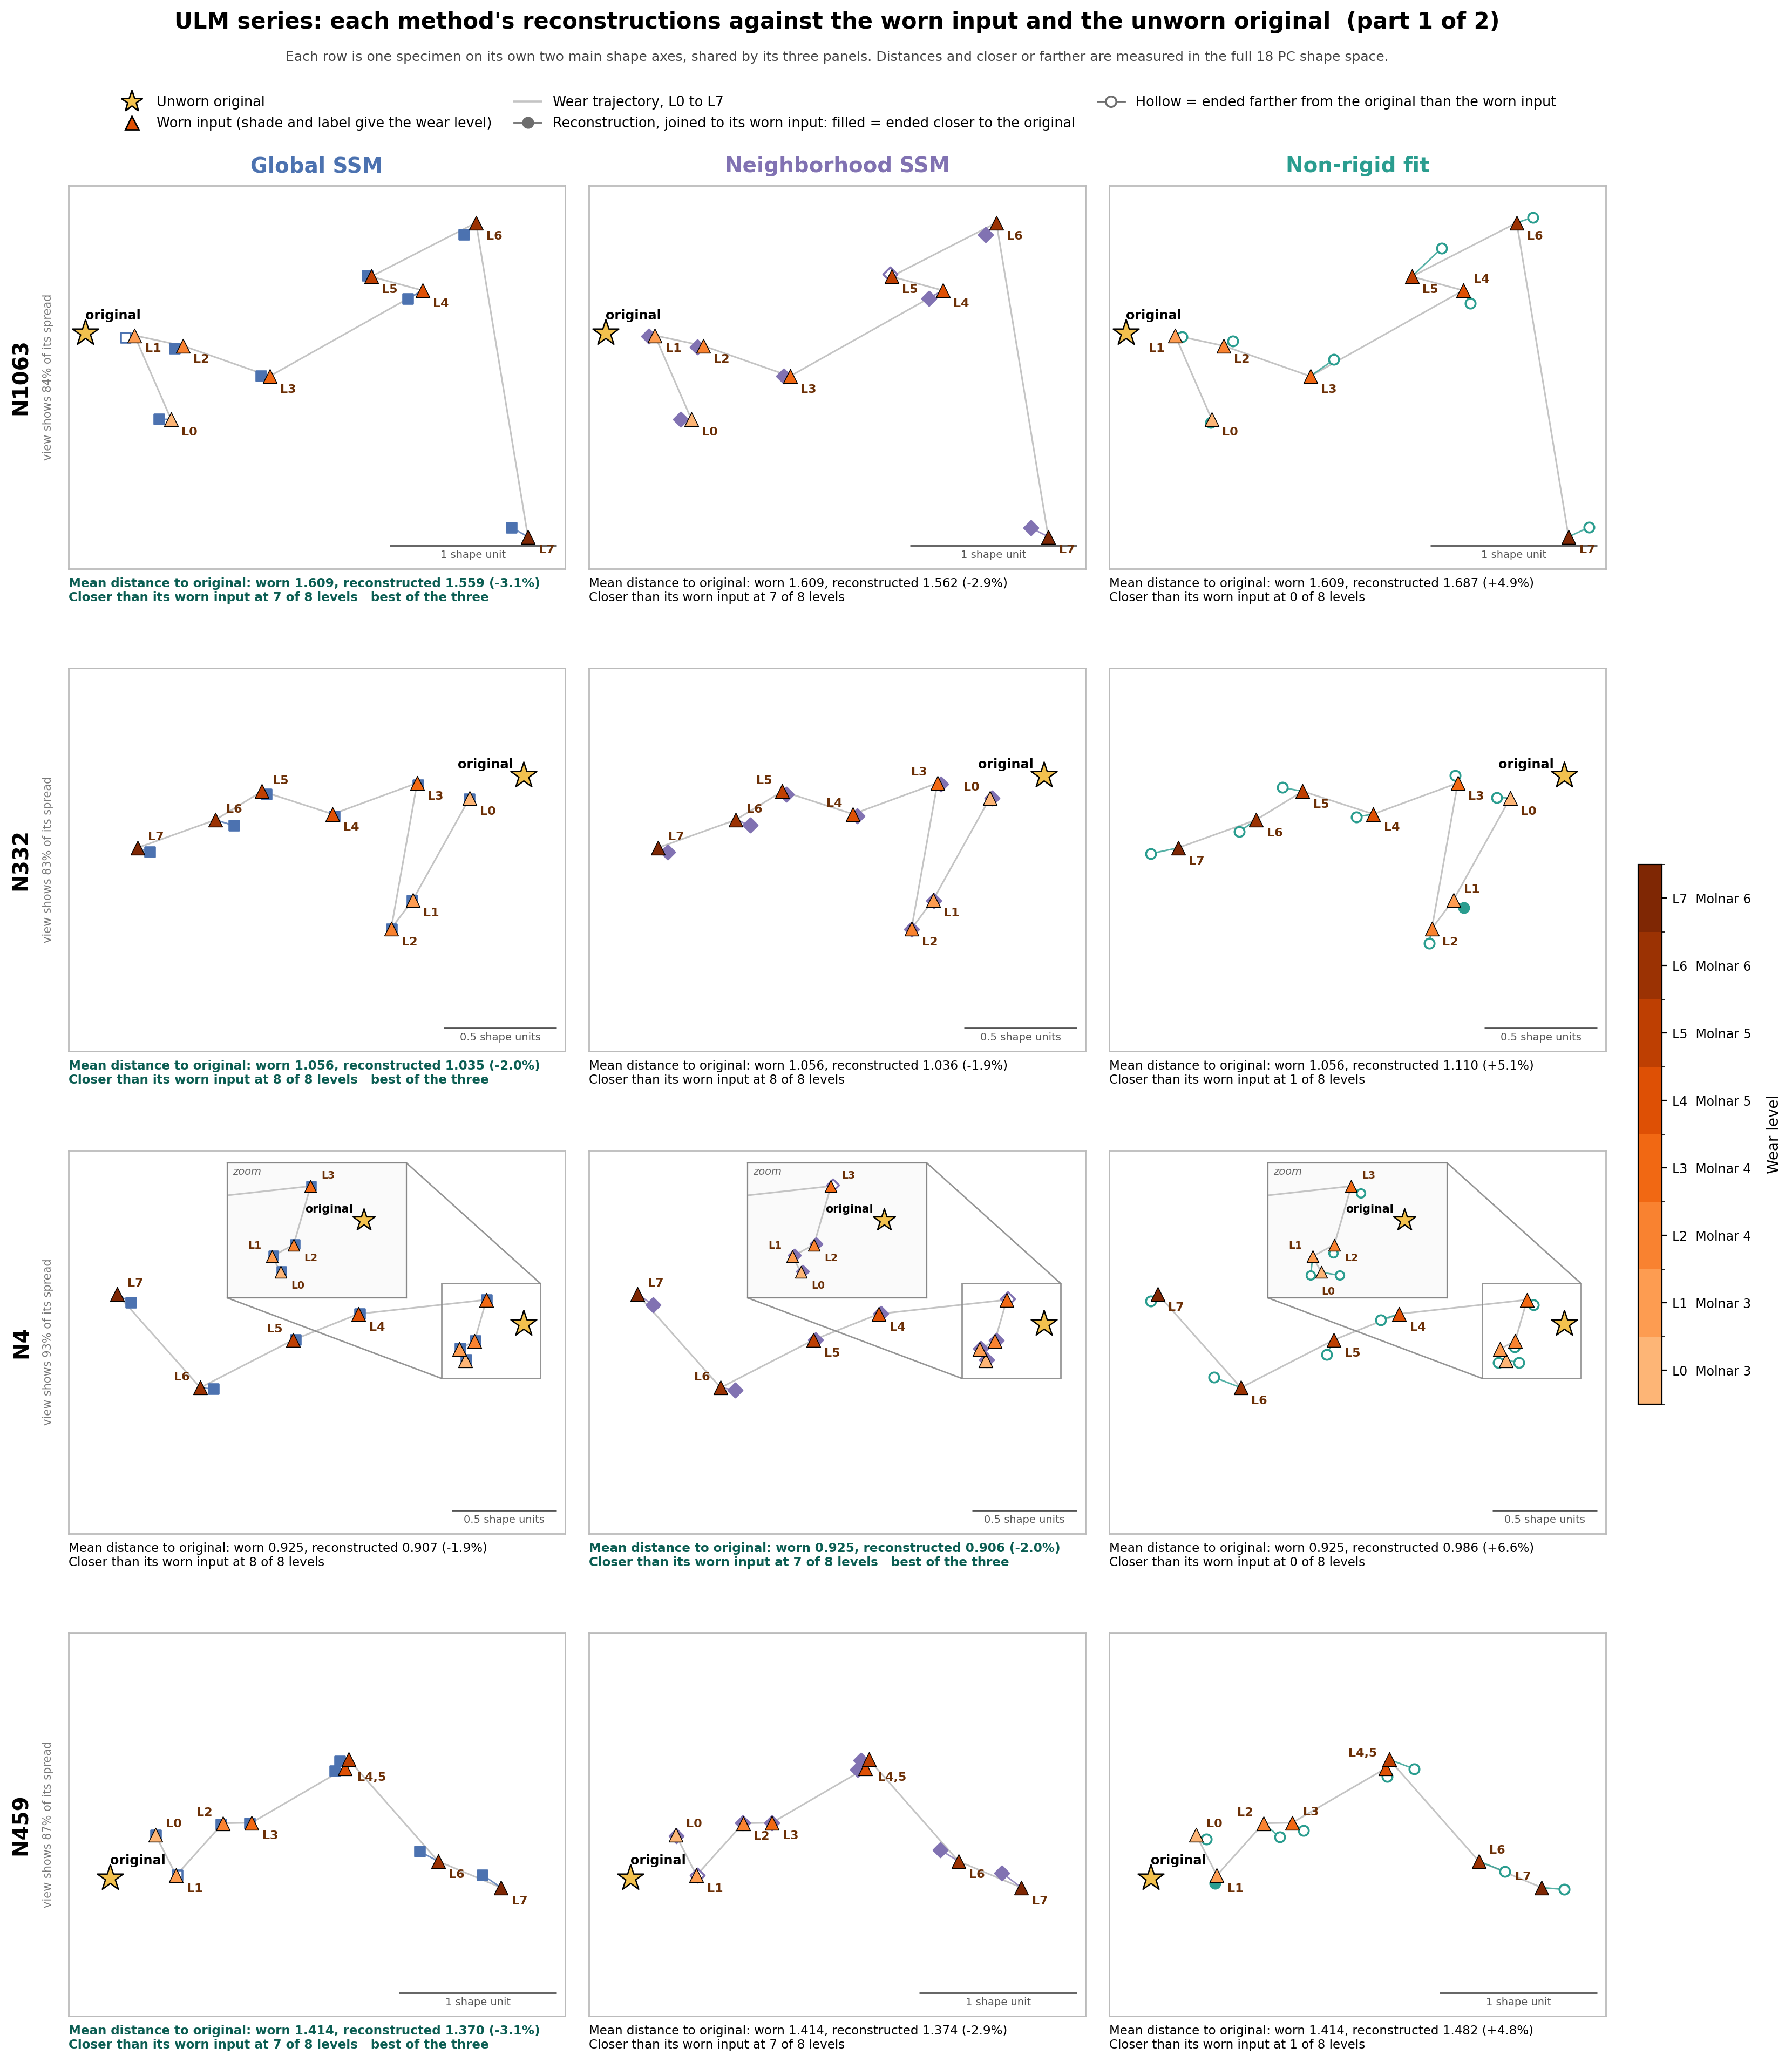
\includegraphics[width=\textwidth]{fig_shape_methods_ulm_part1.png}
\caption{Where each reconstruction lands in shape space, ULM series, specimens
  N1063, N332, N4 and N459. Layout and encoding are as in
  Figure~\ref{fig:shape_edj}; distances use the 18-component ULM shape space
  (\S\ref{sec:shapespace}). The per-specimen axes capture 84\%, 83\%, 93\% and 87\%
  of the spread, respectively. Scale bars differ between rows, so compare
  specimens using the distances printed under each panel.}
\label{fig:shape_ulm1}
\end{figure}

\clearpage

\begin{figure}[H]
\centering
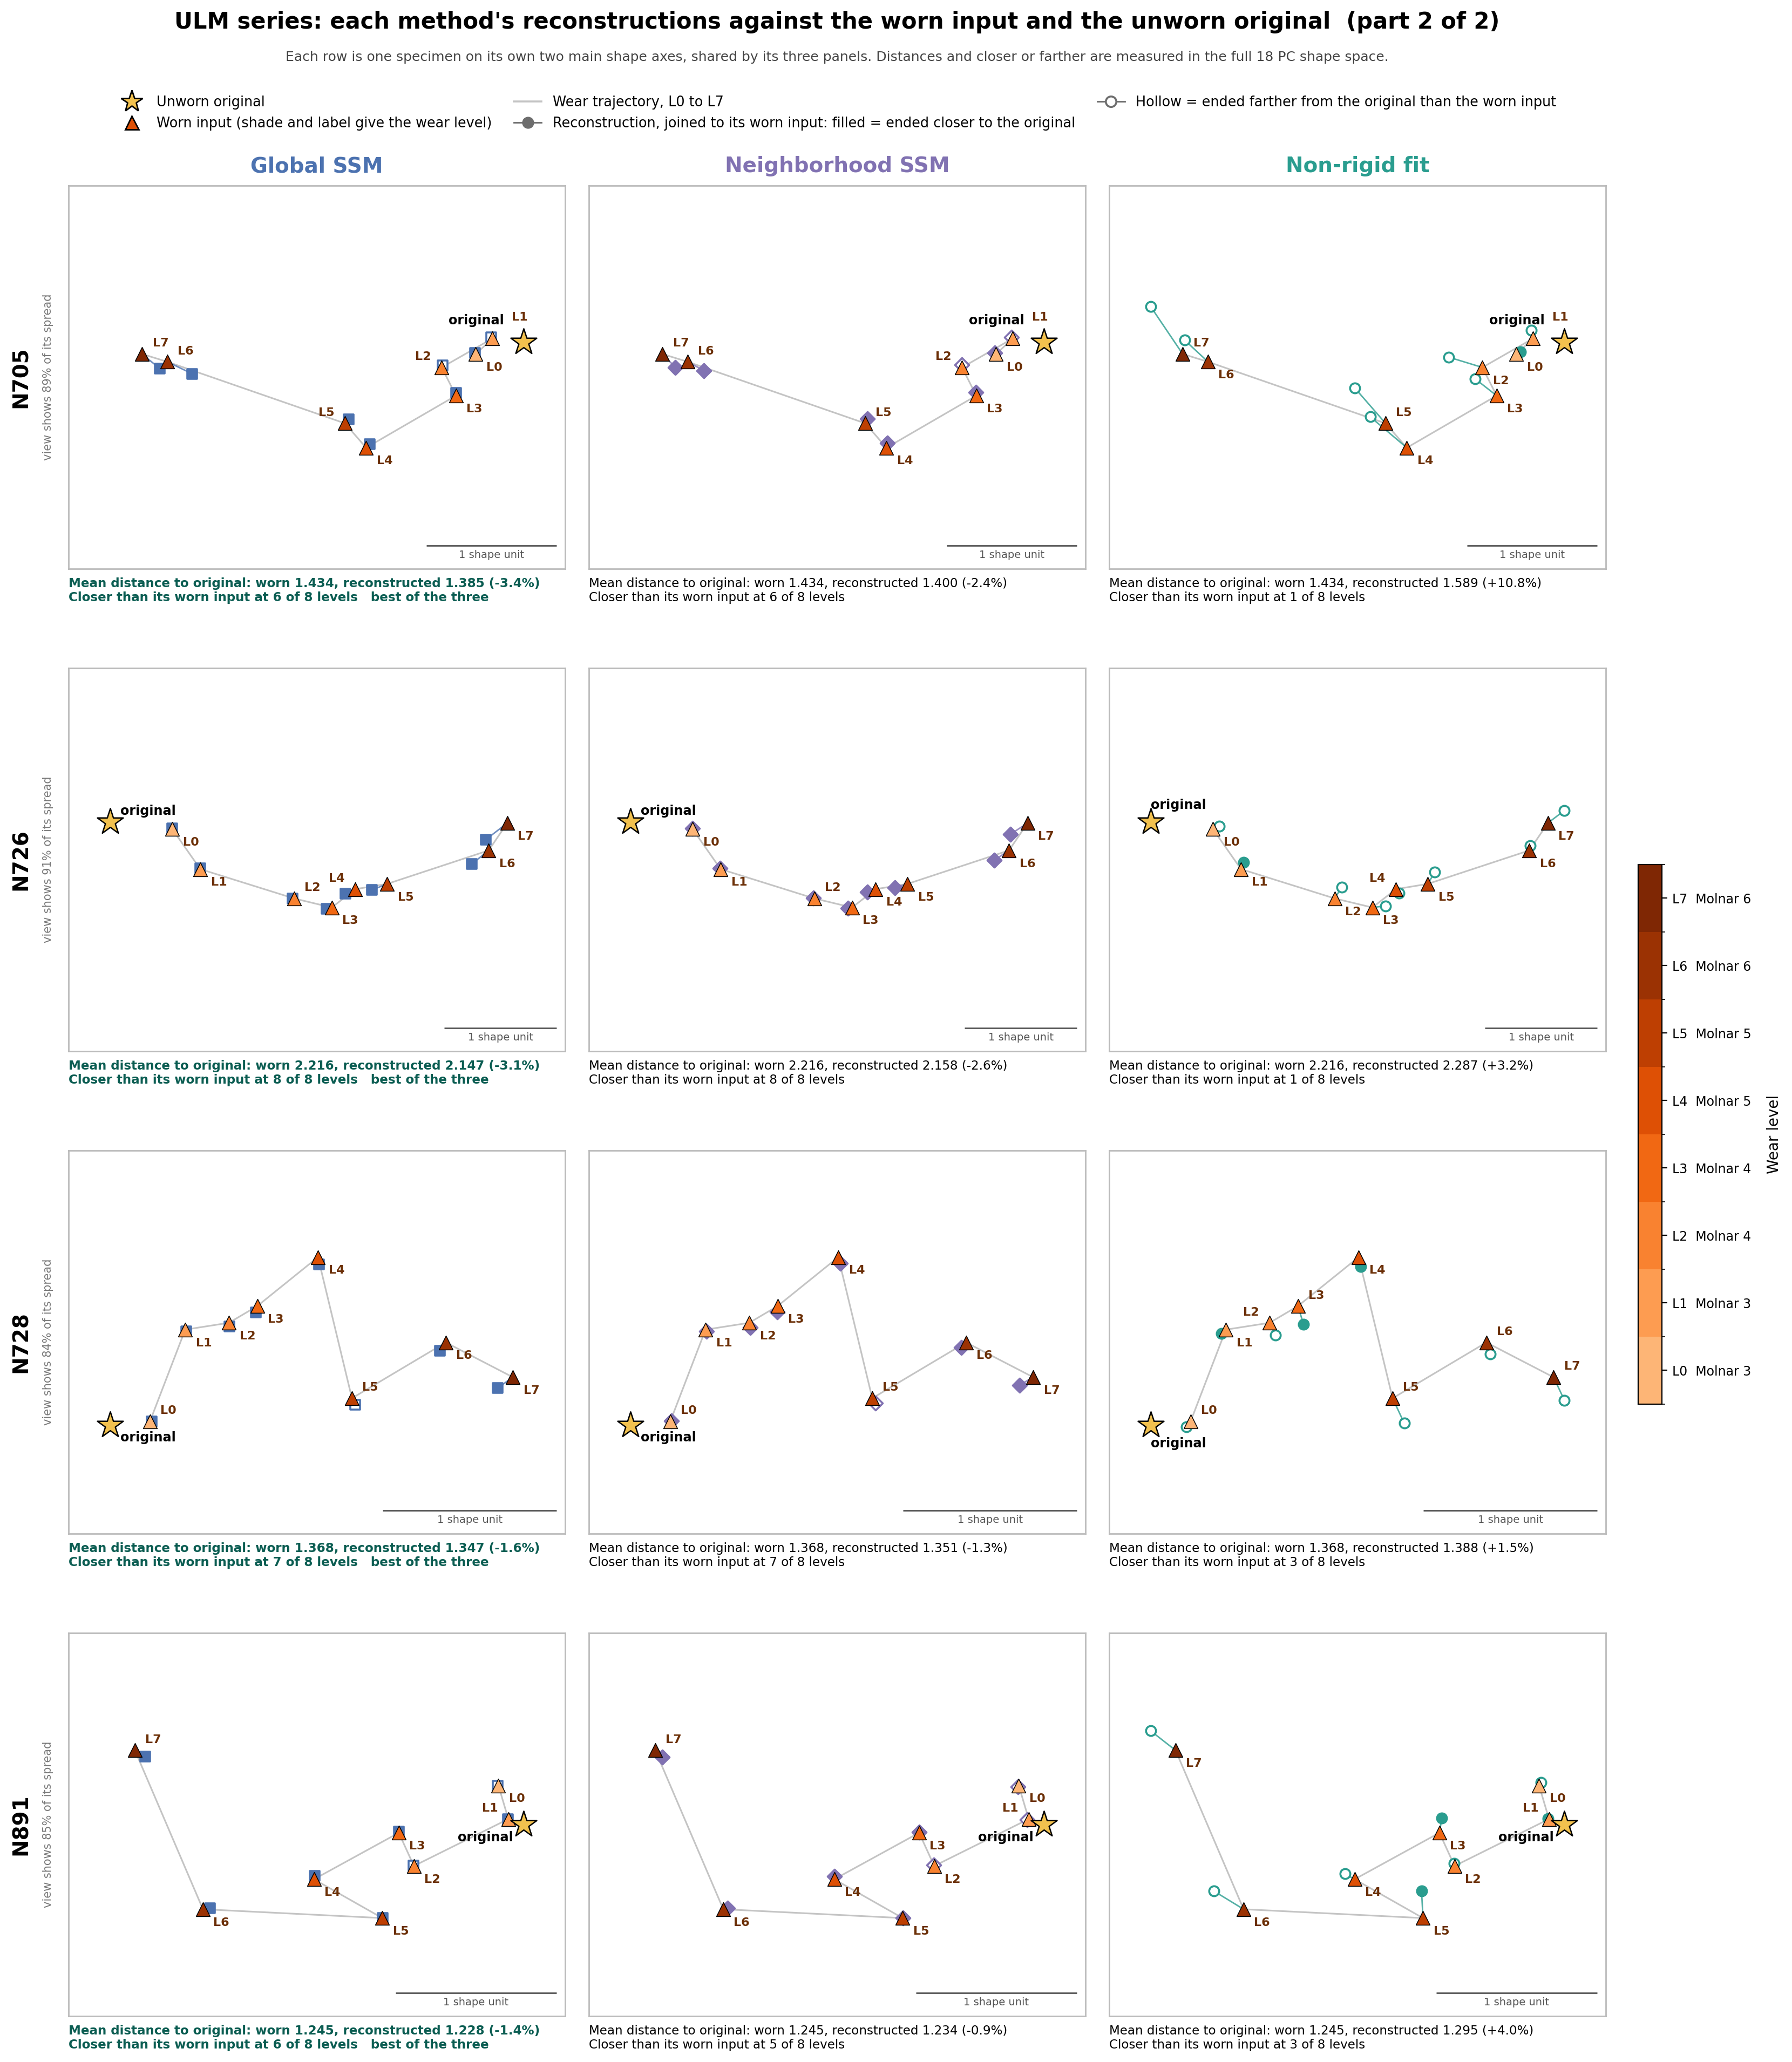
\includegraphics[width=\textwidth]{fig_shape_methods_ulm_part2.png}
\caption{Where each reconstruction lands in shape space, ULM series, specimens
  N705, N726, N728 and N891. Layout and encoding are as in
  Figure~\ref{fig:shape_edj}; distances use the 18-component ULM shape space. The
  per-specimen axes capture 89\%, 91\%, 84\% and 85\% of the spread,
  respectively. Scale bars differ between rows, so compare specimens using the
  distances printed under each panel.}
\label{fig:shape_ulm2}
\end{figure}

\clearpage

\begin{figure}[H]
\centering
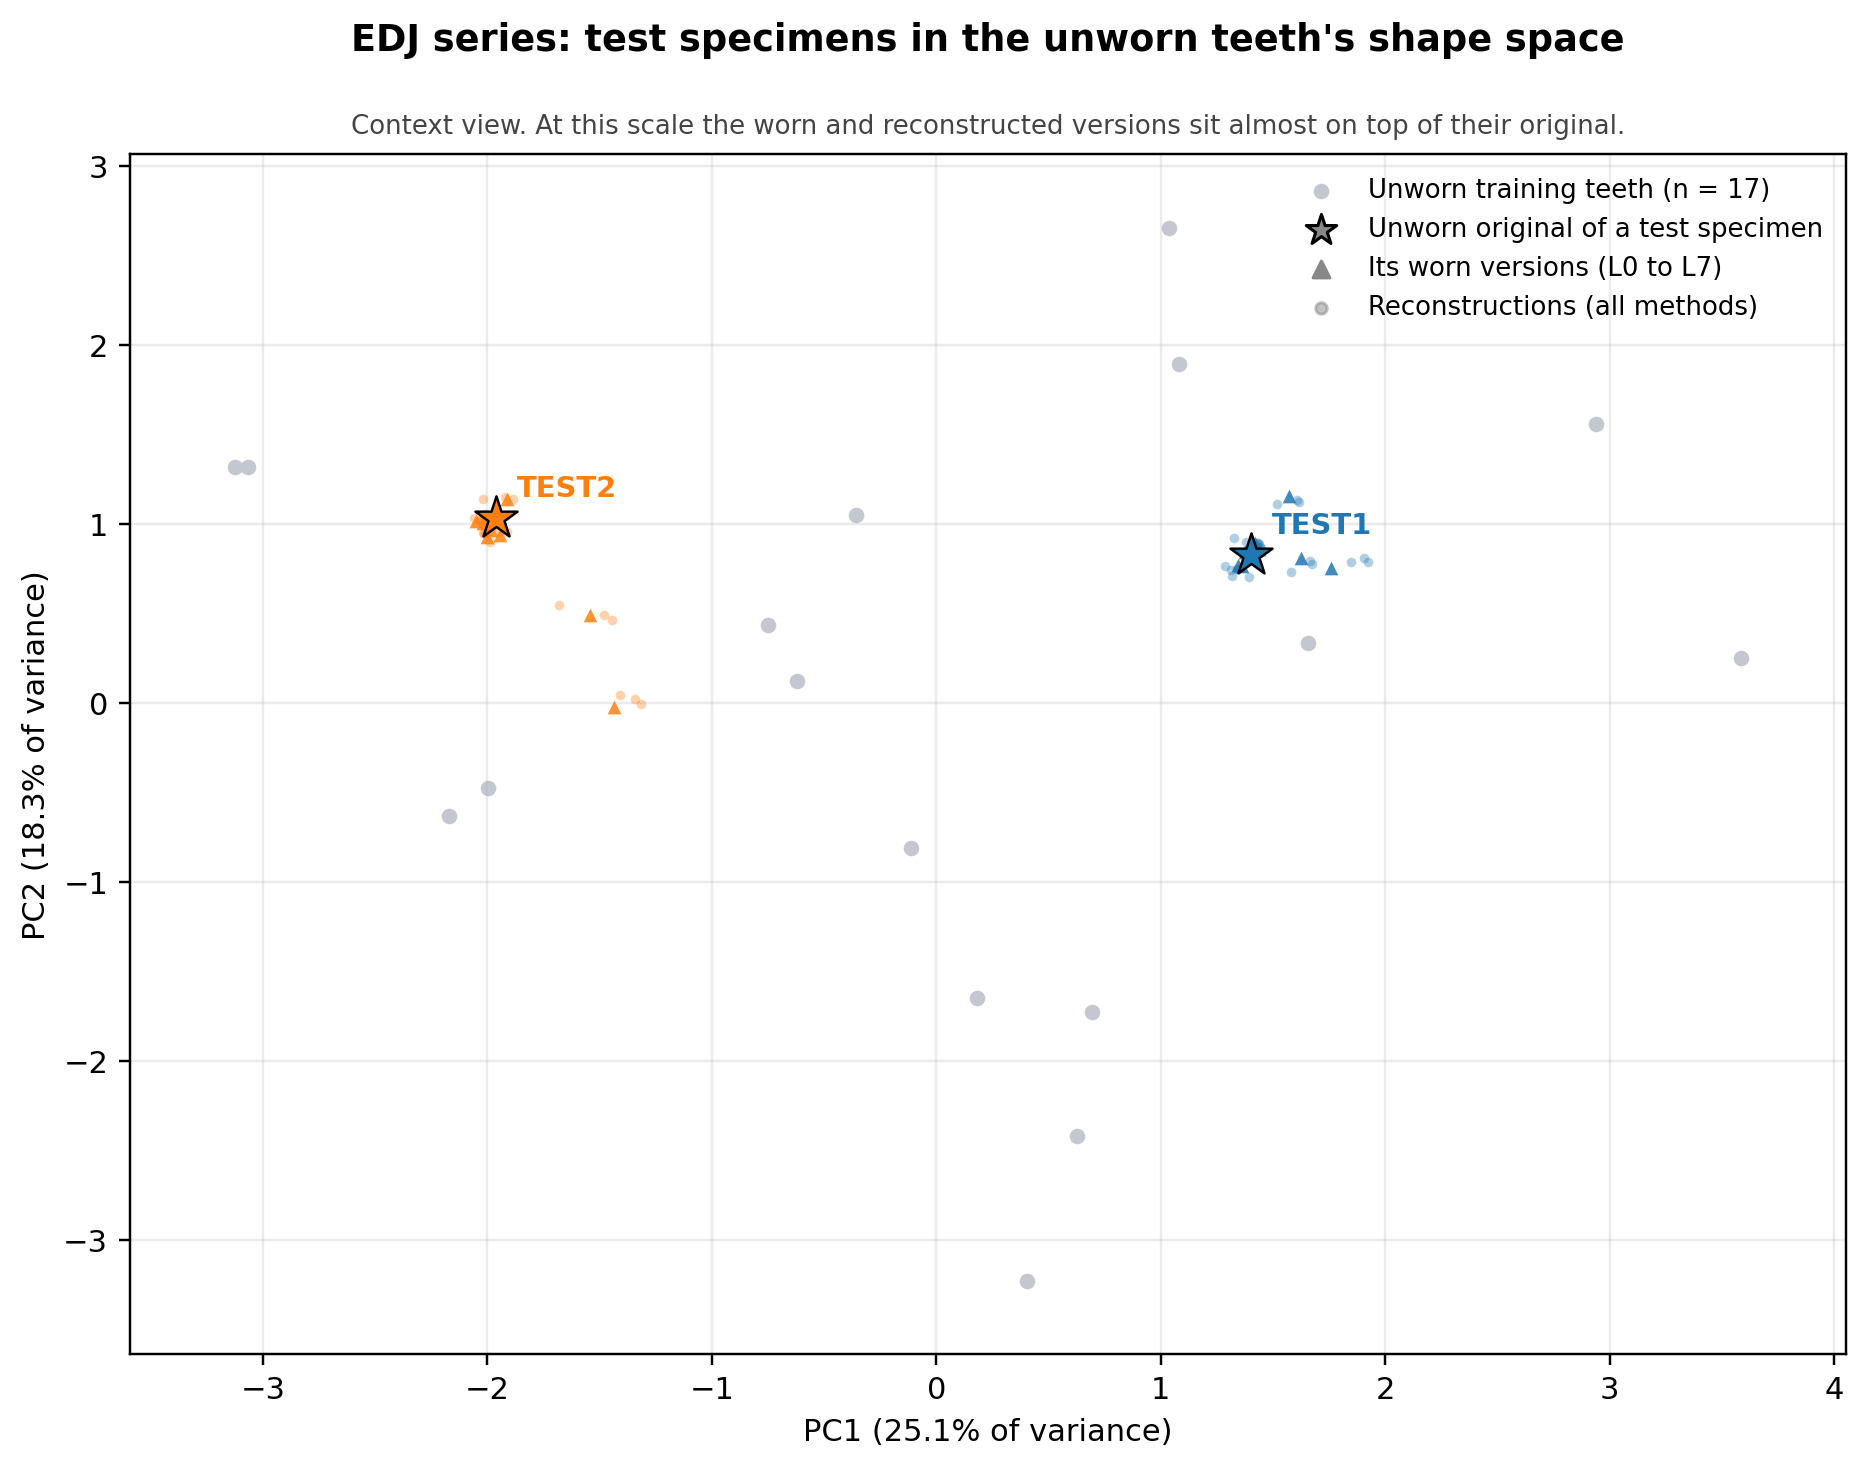
\includegraphics[width=0.66\textwidth]{fig_shape_overview_edj.png}
\caption{EDJ test specimens in the shape space of the unworn training teeth,
  shown on its first two principal components (25.1\% and 18.3\% of the variance).
  Grey points are the 17 training teeth that define the space; \code{n0307} is
  excluded (\S\ref{sec:regcheck}). Stars are the unworn originals of TEST1 and
  TEST2, triangles are their worn inputs and small dots are the reconstructions
  from all three methods. At this scale worn inputs and reconstructions cluster
  around their original. These two components capture only 4\% (TEST1) and 11\%
  (TEST2) of each specimen's own spread, which is why
  Figure~\ref{fig:shape_edj} uses per-specimen axes.}
\label{fig:overview_edj}
\end{figure}

\begin{figure}[H]
\centering
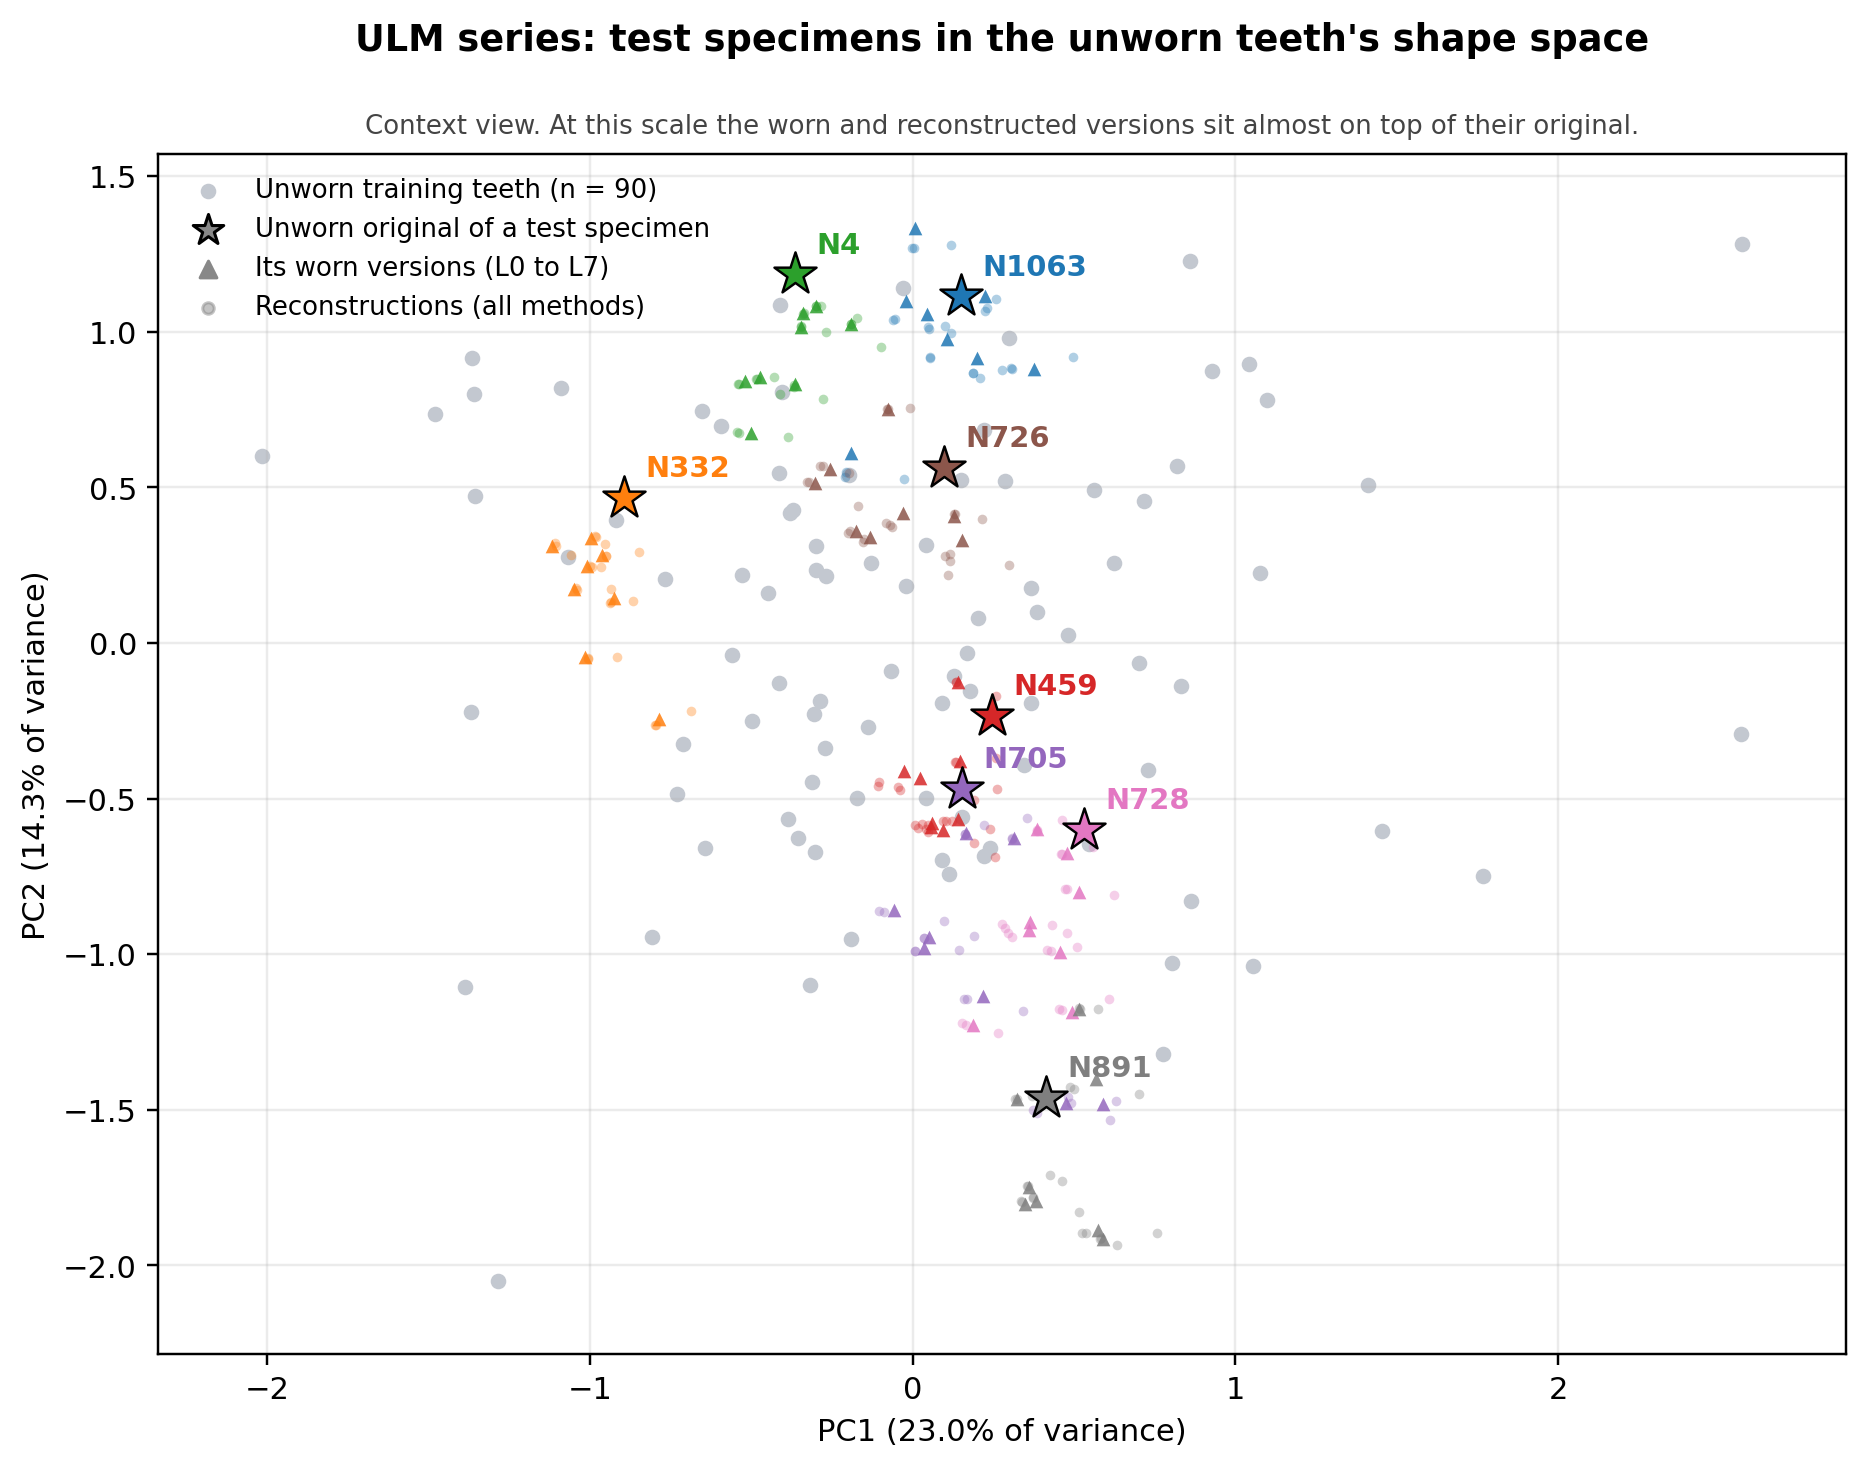
\includegraphics[width=0.66\textwidth]{fig_shape_overview_ulm.png}
\caption{ULM test specimens in the shape space of the 90 unworn training teeth,
  shown on its first two principal components (23.0\% and 14.3\% of the variance).
  Encoding is as in Figure~\ref{fig:overview_edj}. The training teeth form a
  single, continuous cloud and the eight test specimens fall within it. (Before the
  registration check, the training teeth formed two groups along the first
  component; those groups were teeth registered half a turn apart,
  \S\ref{sec:regcheck}.) Worn inputs and reconstructions stay near their
  originals, although the heavily worn inputs of some specimens, such as N332 and
  N891, move noticeably. These two components capture only 4 to 13\% of each
  specimen's own spread, which is why the per-specimen figures use their own
  axes.}
\label{fig:overview_ulm}
\end{figure}

\end{document}
